% Options for packages loaded elsewhere
% Options for packages loaded elsewhere
\PassOptionsToPackage{unicode}{hyperref}
\PassOptionsToPackage{hyphens}{url}
\PassOptionsToPackage{dvipsnames,svgnames,x11names}{xcolor}
%
\documentclass[
  letterpaper,
  DIV=11,
  numbers=noendperiod]{scrreprt}
\usepackage{xcolor}
\usepackage{amsmath,amssymb}
\setcounter{secnumdepth}{5}
\usepackage{iftex}
\ifPDFTeX
  \usepackage[T1]{fontenc}
  \usepackage[utf8]{inputenc}
  \usepackage{textcomp} % provide euro and other symbols
\else % if luatex or xetex
  \usepackage{unicode-math} % this also loads fontspec
  \defaultfontfeatures{Scale=MatchLowercase}
  \defaultfontfeatures[\rmfamily]{Ligatures=TeX,Scale=1}
\fi
\usepackage{lmodern}
\ifPDFTeX\else
  % xetex/luatex font selection
\fi
% Use upquote if available, for straight quotes in verbatim environments
\IfFileExists{upquote.sty}{\usepackage{upquote}}{}
\IfFileExists{microtype.sty}{% use microtype if available
  \usepackage[]{microtype}
  \UseMicrotypeSet[protrusion]{basicmath} % disable protrusion for tt fonts
}{}
\makeatletter
\@ifundefined{KOMAClassName}{% if non-KOMA class
  \IfFileExists{parskip.sty}{%
    \usepackage{parskip}
  }{% else
    \setlength{\parindent}{0pt}
    \setlength{\parskip}{6pt plus 2pt minus 1pt}}
}{% if KOMA class
  \KOMAoptions{parskip=half}}
\makeatother
% Make \paragraph and \subparagraph free-standing
\makeatletter
\ifx\paragraph\undefined\else
  \let\oldparagraph\paragraph
  \renewcommand{\paragraph}{
    \@ifstar
      \xxxParagraphStar
      \xxxParagraphNoStar
  }
  \newcommand{\xxxParagraphStar}[1]{\oldparagraph*{#1}\mbox{}}
  \newcommand{\xxxParagraphNoStar}[1]{\oldparagraph{#1}\mbox{}}
\fi
\ifx\subparagraph\undefined\else
  \let\oldsubparagraph\subparagraph
  \renewcommand{\subparagraph}{
    \@ifstar
      \xxxSubParagraphStar
      \xxxSubParagraphNoStar
  }
  \newcommand{\xxxSubParagraphStar}[1]{\oldsubparagraph*{#1}\mbox{}}
  \newcommand{\xxxSubParagraphNoStar}[1]{\oldsubparagraph{#1}\mbox{}}
\fi
\makeatother


\usepackage{longtable,booktabs,array}
\usepackage{calc} % for calculating minipage widths
% Correct order of tables after \paragraph or \subparagraph
\usepackage{etoolbox}
\makeatletter
\patchcmd\longtable{\par}{\if@noskipsec\mbox{}\fi\par}{}{}
\makeatother
% Allow footnotes in longtable head/foot
\IfFileExists{footnotehyper.sty}{\usepackage{footnotehyper}}{\usepackage{footnote}}
\makesavenoteenv{longtable}
\usepackage{graphicx}
\makeatletter
\newsavebox\pandoc@box
\newcommand*\pandocbounded[1]{% scales image to fit in text height/width
  \sbox\pandoc@box{#1}%
  \Gscale@div\@tempa{\textheight}{\dimexpr\ht\pandoc@box+\dp\pandoc@box\relax}%
  \Gscale@div\@tempb{\linewidth}{\wd\pandoc@box}%
  \ifdim\@tempb\p@<\@tempa\p@\let\@tempa\@tempb\fi% select the smaller of both
  \ifdim\@tempa\p@<\p@\scalebox{\@tempa}{\usebox\pandoc@box}%
  \else\usebox{\pandoc@box}%
  \fi%
}
% Set default figure placement to htbp
\def\fps@figure{htbp}
\makeatother





\setlength{\emergencystretch}{3em} % prevent overfull lines

\providecommand{\tightlist}{%
  \setlength{\itemsep}{0pt}\setlength{\parskip}{0pt}}



 


\KOMAoption{captions}{tableheading}
\makeatletter
\@ifpackageloaded{bookmark}{}{\usepackage{bookmark}}
\makeatother
\makeatletter
\@ifpackageloaded{caption}{}{\usepackage{caption}}
\AtBeginDocument{%
\ifdefined\contentsname
  \renewcommand*\contentsname{Table of contents}
\else
  \newcommand\contentsname{Table of contents}
\fi
\ifdefined\listfigurename
  \renewcommand*\listfigurename{List of Figures}
\else
  \newcommand\listfigurename{List of Figures}
\fi
\ifdefined\listtablename
  \renewcommand*\listtablename{List of Tables}
\else
  \newcommand\listtablename{List of Tables}
\fi
\ifdefined\figurename
  \renewcommand*\figurename{Figure}
\else
  \newcommand\figurename{Figure}
\fi
\ifdefined\tablename
  \renewcommand*\tablename{Table}
\else
  \newcommand\tablename{Table}
\fi
}
\@ifpackageloaded{float}{}{\usepackage{float}}
\floatstyle{ruled}
\@ifundefined{c@chapter}{\newfloat{codelisting}{h}{lop}}{\newfloat{codelisting}{h}{lop}[chapter]}
\floatname{codelisting}{Listing}
\newcommand*\listoflistings{\listof{codelisting}{List of Listings}}
\makeatother
\makeatletter
\makeatother
\makeatletter
\@ifpackageloaded{caption}{}{\usepackage{caption}}
\@ifpackageloaded{subcaption}{}{\usepackage{subcaption}}
\makeatother
\usepackage{bookmark}
\IfFileExists{xurl.sty}{\usepackage{xurl}}{} % add URL line breaks if available
\urlstyle{same}
\hypersetup{
  pdftitle={Sailcraft},
  pdfauthor={Chris Thompson},
  colorlinks=true,
  linkcolor={blue},
  filecolor={Maroon},
  citecolor={Blue},
  urlcolor={Blue},
  pdfcreator={LaTeX via pandoc}}


\title{Sailcraft}
\usepackage{etoolbox}
\makeatletter
\providecommand{\subtitle}[1]{% add subtitle to \maketitle
  \apptocmd{\@title}{\par {\large #1 \par}}{}{}
}
\makeatother
\subtitle{The history and design of the racing dinghy}
\author{Chris Thompson}
\date{2026-04-29}
\begin{document}
\maketitle

\renewcommand*\contentsname{Table of contents}
{
\hypersetup{linkcolor=}
\setcounter{tocdepth}{2}
\tableofcontents
}

\bookmarksetup{startatroot}

\chapter*{Preface}\label{preface}
\addcontentsline{toc}{chapter}{Preface}

\markboth{Preface}{Preface}

This is a Quarto book.

To learn more about Quarto books visit
\url{https://quarto.org/docs/books}.

I am attempting to render this for publication.

Happy birthday Chris!

\bookmarksetup{startatroot}

\chapter*{Introduction}\label{introduction}
\addcontentsline{toc}{chapter}{Introduction}

\markboth{Introduction}{Introduction}

The SailCraft blog was really born years ago, when I realised that no
one had tried to tell the story of the racing dinghy and the forces that
shaped it. It's a complex tale; a web of interaction between factors
such as emerging technologies, differences in geography and economies,
the physics of wind and water, real estate and liquor laws, the width of
an Austin A40 sedan and an English seaside laneway, and changing gender
roles. It's a tale that has spawned many myths, often ones about
conservatives stifling development, but where the reality has few such
villains and many heroes. \footnote{and a few heroines, but, sadly, not
  too many.}

\pandocbounded{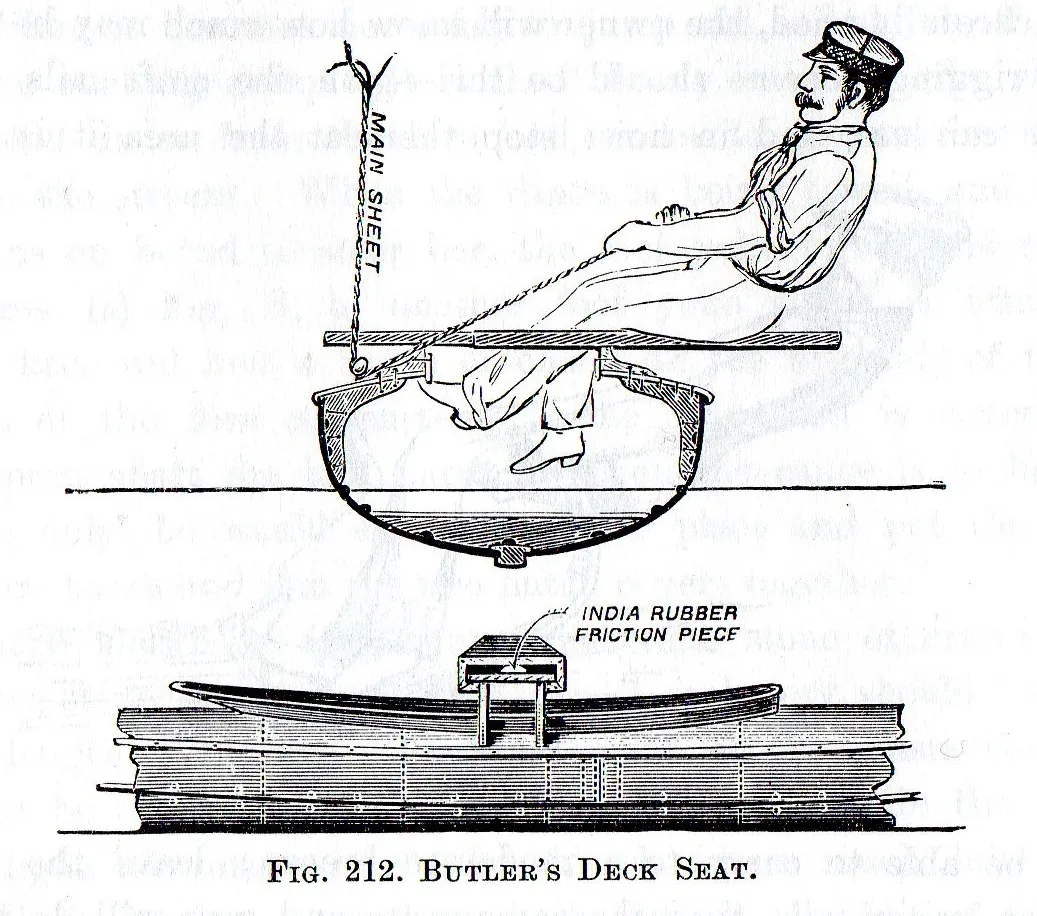
\includegraphics[keepaspectratio]{images/dixon-kemp-sliding-seat1.png}}

This is an ideal time to tell this story. The arrival of online archives
allows us to find information that has been hidden away in ancient
newspapers and rare mouldering books. It's a time when even the shyest
dinghy designer can be coaxed into giving priceless nuggets of
information over email. Many of the world's top dinghy creators,
including Paul Bieker, Frank and Julian Bethwaite, Ian Bruce, Rob Brown,
Steve Clark, Stu Friezer, Mike Jackson, Bruce Kirby, Andrew McDougal,
Phil Morrison, Andy Paterson and many more, have been happy to be
interviewed for this project.

\pandocbounded{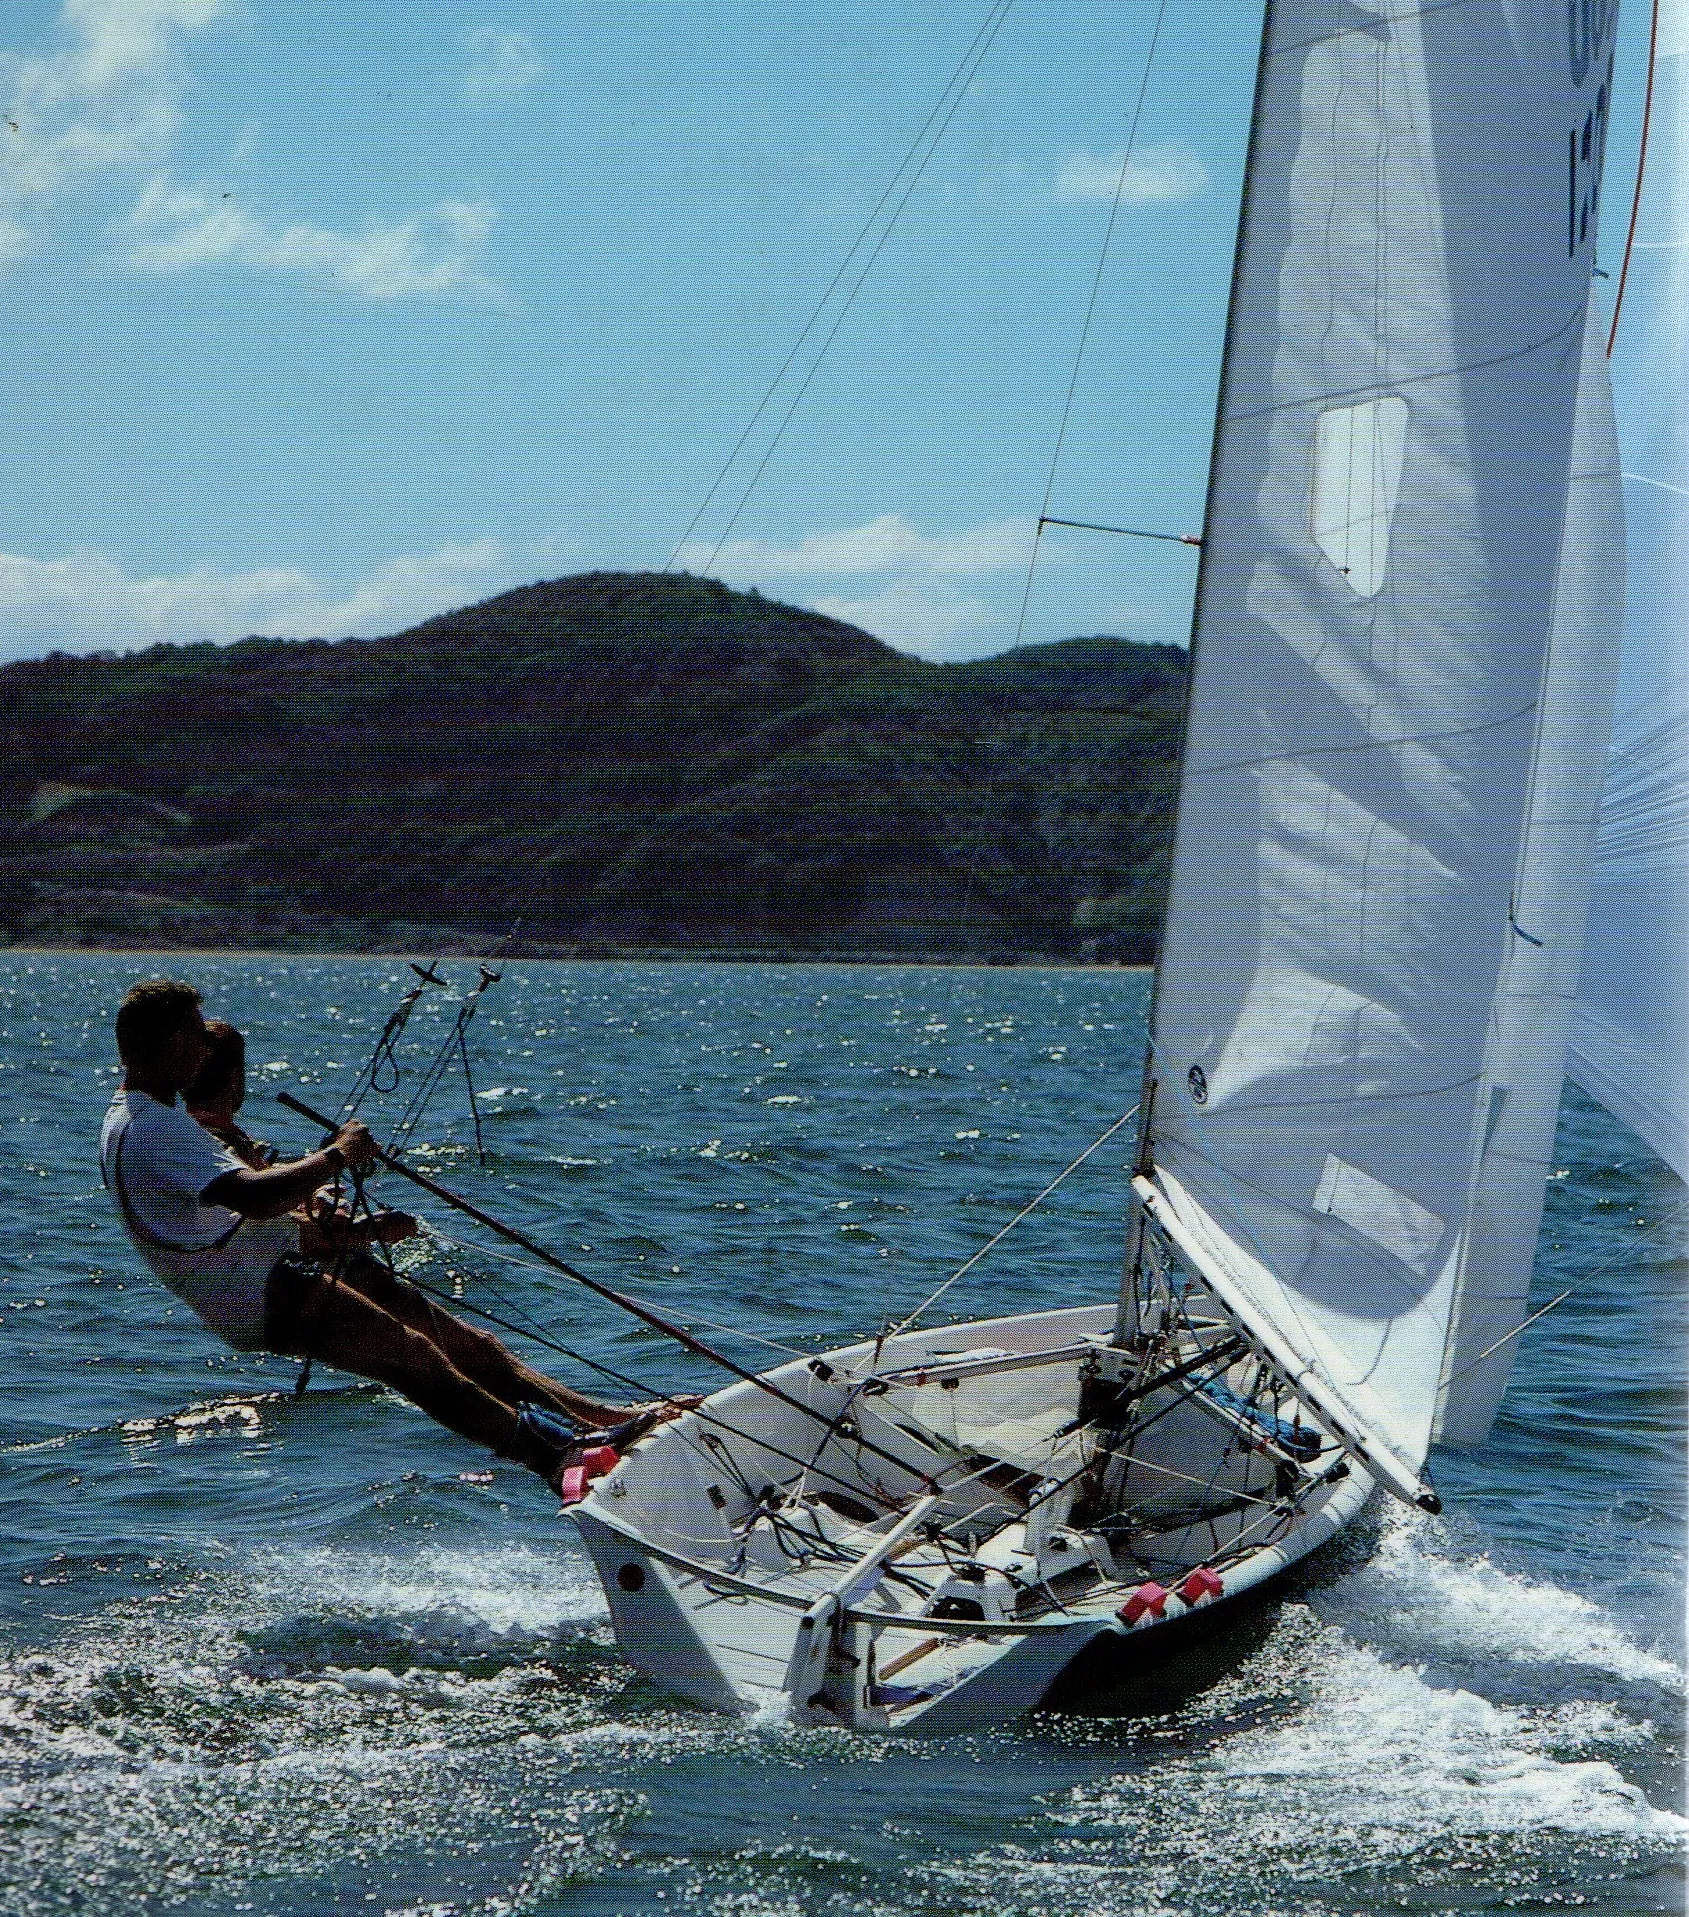
\includegraphics[keepaspectratio]{images/int-14-back-cover.png}}

The same changes in technology have also delayed SailCraft by years.
I've been waiting for digital publishing to develop to the stage where
it can provide images of boat designs and photographs well enough to
show intricate details like the hull lines of a Bieker 14, or the
workmanship of an Uffa Fox classic. Such technology still isn't here,
and sadly my ability to write well still hasn't returned, so I have
turned to this blog to pass on the information that so many people have
helped me to gather. Many thanks to them and the many other people who
have given their time and knowledge in the past, and my apologies for
the long delay.

SailCraft comes in three parts. Part 1 is a history of the development
of the racing dinghy (and the bigger boats that influenced them) from
the 18th century to the present day. Part 2 is an examination of the
design principles and philosophies that dinghy designers follow. Part 3
is an examination of individual classes and types and their design and
development.

\pandocbounded{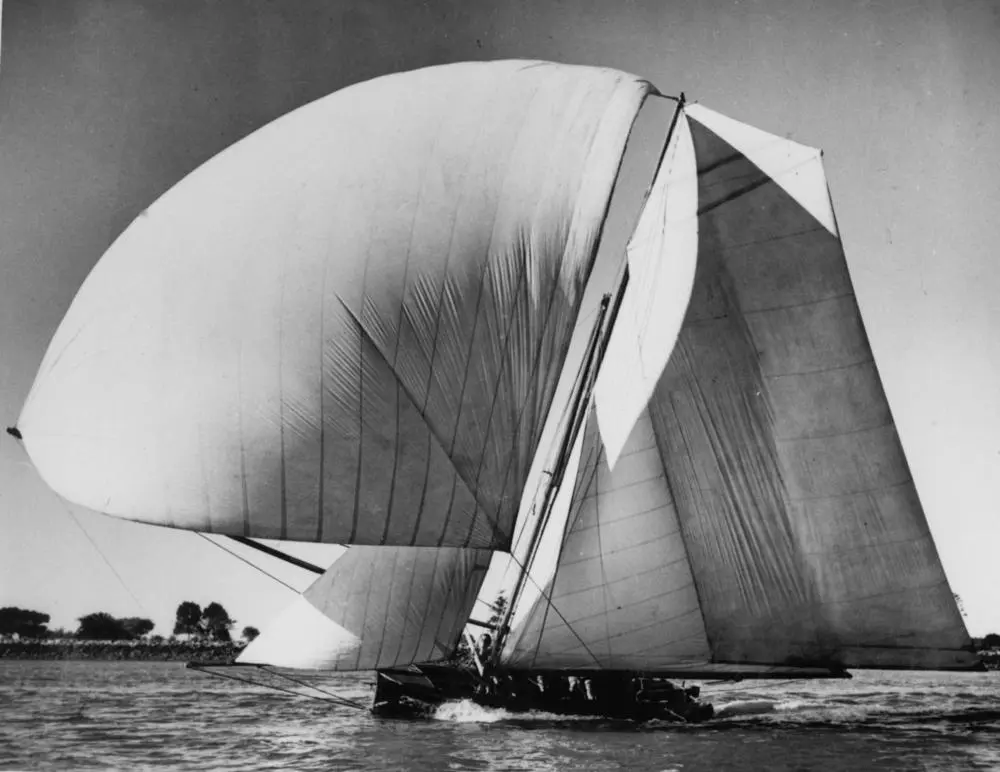
\includegraphics[keepaspectratio]{images/intro/yachting_queensland_1940s.png}}

This blog is concentrating on Part 1 at first, starting from the 1700s,
when the first racing centreboarders arrived. Part 1 is generally being
posted in chronological order, but some out-of-sequence posts will be
put up at times. Some sections from Parts 2 and 3 will also be posted
out of order at times.

There are still many gaps in the story of the racing dinghy and its
design. I would love to hear from anyone who wants to provide any
information, comment or corrections.

Chris Thompson

\bookmarksetup{startatroot}

\chapter{``The sliding keels that took advantage'' - the dawn of the
racing
centreboarder}\label{the-sliding-keels-that-took-advantage---the-dawn-of-the-racing-centreboarder}

\begin{figure}[H]

{\centering \pandocbounded{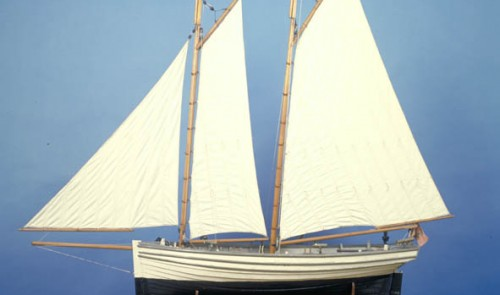
\includegraphics[keepaspectratio]{images/peggymodel.jpg}}

}

\caption{A model of Peggy of Castletown -- the victor in the first known
race involving open centreboard boats.}

\end{figure}%

Like all good sea stories, the history of the racing dinghy starts with
smugglers, a fortune, a struggle for the hand of a maiden, cannons,
islands, and a mutiny. The man who brought them all together was John
Christian of the Isle of Man and England's Lake District -- the man who
organised what seems to have been the first race for small centreboard
boats.

John Christian was a political and social reformer, an agricultural
innovator, and it was said, father to half the children in his town. As
you'd expect from a powerful and passionate man in that part of the
world, John Christian was also a sailor. In 1780, he had the 25'6″/7.77m
long Margaret built in nearby port of Whitehaven. With her open cockpit,
long, shallow keel and small lug rig, Margaret looks generally similar
to other small boats of her era; heavily built, canoe sterned and rather
slow.

Two years after he launched Margaret, John Christian married his cousin
and ward, Isabelle Curwen. The marriage didn't just give John Christian
Curwen (as he became known) a new name and an apparently happy marriage;
it also gave him Isabelle's inheritance. John Christian Curwen spent
some of that fortune in the best possible way -- by buying a waterfront
estate on England's famously beautiful Lake Windermere (including the
famous Belle Isle, named after his bride) and establishing the first
Windermere regatta. \footnote{Much of this information on Peggy is from
  the site of the Castletown municipal site; see
  http://www.castletown.org.im/heritage/nm\_peggy.html}

And what of Curwen's cousin Fletcher, the man who may have been his
rival for Isabelle's affections? It's said that he went away to sea to
ease his broken heart, and on April 28 1789, the unhappy Fletcher
Christian sparked one of history's greatest small-boat voyages when he
led the mutiny against his commander, Captain William Bligh of the HMS
Bounty, and set him adrift in the ship's launch -- a boat that, save for
her transom stern, looks to be similar in style to Margaret.

\begin{figure}

\begin{minipage}{0.50\linewidth}

\centering{

\pandocbounded{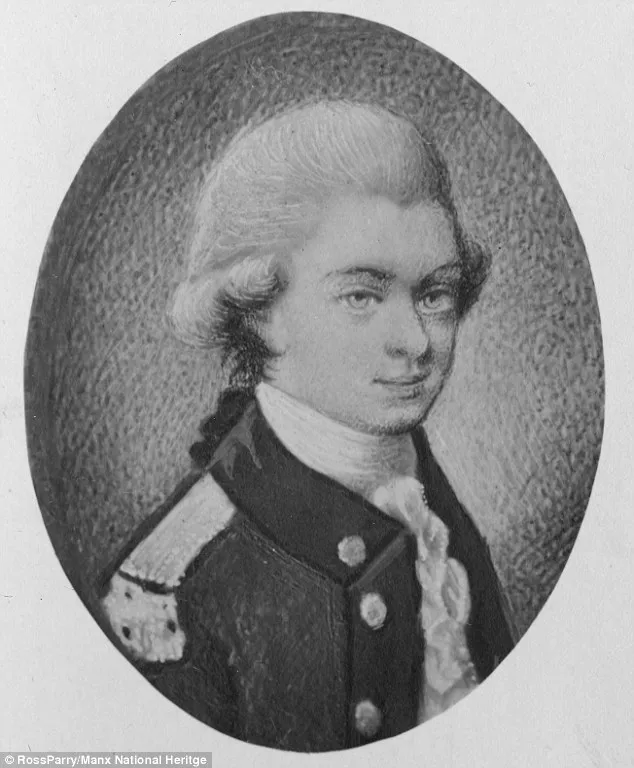
\includegraphics[keepaspectratio]{images/georgequayle.png}}

}

\subcaption{\label{fig-quayle}Quayle}

\end{minipage}%
%
\begin{minipage}{0.50\linewidth}

\centering{

\pandocbounded{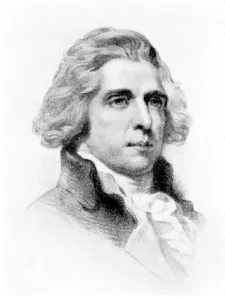
\includegraphics[keepaspectratio]{images/jcurwen2.png}}

}

\subcaption{\label{fig-curwen}Curwen}

\end{minipage}%

\caption{\label{fig-curwenquayle}George Quayle (left) and John Christian
Curwen (right); two brilliant men and rivals in the world's first known
race with open centreboarders.}

\end{figure}%

John Christian Curwen never achieved Fletcher's fame, but he settled
down to a distinguished life of radical politics, social and
agricultural reform, field sports and sailing. In 1796, he entered into
a challenge with his relative George Quayle, a merchant, inventor,
ship-owner, banker, and politician from Douglas on the Isle of Man in
the Irish Sea. Seven years earlier, Quayle had launched the 26'5″/7.77m
long open schooner Peggy. Peggy was used for transportation and as a
workboat for Quayle's business (with perhaps some smuggling on the side)
but Quayle's letters show that she was also a pleasure boat and a joy to
him.

\begin{figure}[H]

{\centering \pandocbounded{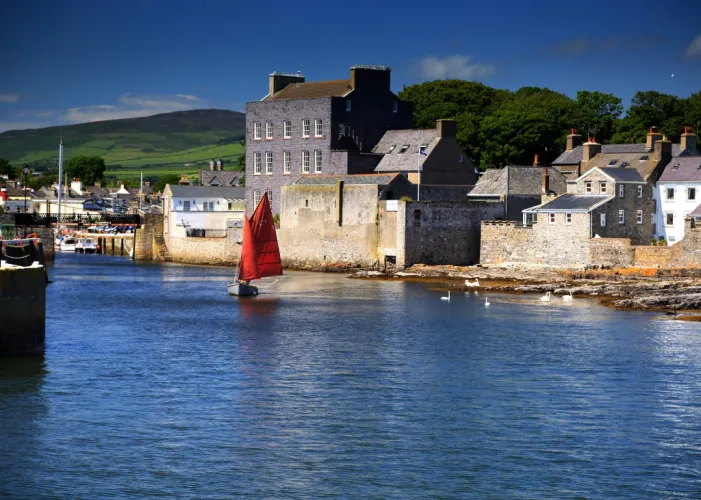
\includegraphics[keepaspectratio]{images/red-sails.png}}

}

\caption{One of the Castletown One Designs sails down the tiny
Castletown Harbour, past Quayle's `Bridge House' -- the large grey
building in the centre. The white sign on the right-hand end of the
house marks the boatshed where Peggy was kept. Photo from Isle of Man
Film}

\end{figure}%

As the noted Irish yachting journalist W M Nixon noted in an excellent
article in Wooden Boat magazine, Quayle's Peggy seems to be a much more
advanced design than Curwen's craft.\footnote{``Meetings with Mature
  Ladies'':- Wooden Boat May/June 1986, p 17.} A rakish-looking boat
with fine lines by the standards of the time, she carried a powerful
schooner rig. She was constructed with clinker or lapstrake planking,
which is normally lighter than the normal carvel hull used by boats like
Margaret.

Peggy is, of course, much bigger than a modern dinghy, but so were many
of the boats that played a part in the early development of the dinghy.
These days most developments trickle up from dinghies to big boats, but
in the early days of dinghy sailing, when rigs and boats were heavy and
stuck in the rut of displacement speeds, small dinghies were all but
ignored. At the dawn of centreboarder sailing, developments trickled
down from bigger boats.

Quayle kept on tinkering with Peggy long after her launch. By 1796 he
had fitted her with two or three examples of the new invention that was
to become the signature of the dinghy -- the ``sliding keel'' or, as we
know it, the centreboard. \footnote{``The Worthies of Cumberland'' Vol
  1, Henry Lonsdale MD, 1867, p 66.}

Like so much other technology, the ``sliding keel'' had been developed
by the military. Captain Schank of the Royal Navy had come up with the
idea in 1774, when he was in charge of building the fleet of small
warships that won the Battle of Lake Champlain during the War of
Independence. Schank's ``sliding keel'' was merely one component of a
theory of hull design that formed a striking contrast to the concepts
behind the normal deep-hulled sailing vessel of the day. Schank and his
patron Lord Percy realised that if vessels ``were built much flatter, so
as to go on the surface and not draw much water, they would sail faster,
and might still be enabled to carry as much sail, and keep up to the
wind, by having their keels descend a greater depth; and that the flat
side of the keel, when presented to the water would make them able to
spread more canvas, and hold the wind better, than in a construction
whereby they present only the circular surface to the water''. The theme
of ``surface sailing'', instead of cutting through the water, was to
become a hallmark of the centeboarder in the next century, and to be
endlessly re-interpreted as boats became lighter and lighter.

Although Schank gave Percy the credit for the ``surface sailing''
concept, it was Schank who conceived of a keel ``that was made movable,
and to be screwed upwards into a trunk, or well formed within the
vessel'' so that the shallow-hulled deep-keeled craft he and Percy
envisaged could still enter shallow waters. The experimental boat that
Schank built for Percy in Boston in 1774 was the first known
``centreboarder.''

\begin{figure}

\begin{minipage}{\linewidth}

\centering{

\pandocbounded{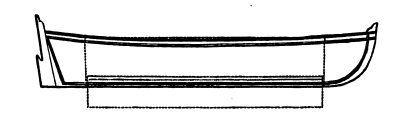
\includegraphics[keepaspectratio]{images/chapter1/one-centreboard-schank-boat.png}}

}

\subcaption{\label{fig-oneC}}

\end{minipage}%
\newline
\begin{minipage}{\linewidth}

\centering{

\pandocbounded{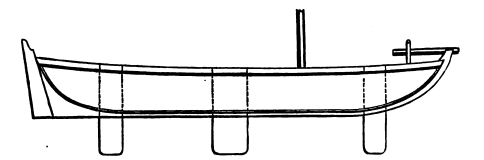
\includegraphics[keepaspectratio]{images/chapter1/three-centreboard-schank-boat-cropped.png}}

}

\subcaption{\label{fig-threeC}}

\end{minipage}%

\caption{\label{fig-centreboards}Top: The first ``centreboarder'',
Schank's ``sliding keel'' boat of 1775. The long single ``keel'' was
replaced by three keels in the next experimental craft (bottom), which
allowed the boat's helm to be balanced for different points of sail.
Peggy was fitted with a similar arrangement some time after her
construction. Drawings from Dixon Kemp's Manual of Yacht and Boat
Sailing.}

\end{figure}%

The Royal Navy, although understandably distracted by wars with the USA
and France, launched three experimental ships by 1796, and later
followed her up with several classes of ``sliding keel'' brigs. The
Navy's enthusiasm for sliding keels seems to have faded when experience
with vessels like the brig HMS Lady Nelson proved that 18th century
technology was not up to the task of making a large centreboard that
would not break, and that a ship with a broken ``sliding keel'' was even
slower upwind than a normal square rigger. It was a classic
demonstration of the fact that innovation in design is inextricably
linked with material technology.

\begin{figure}[H]

{\centering \pandocbounded{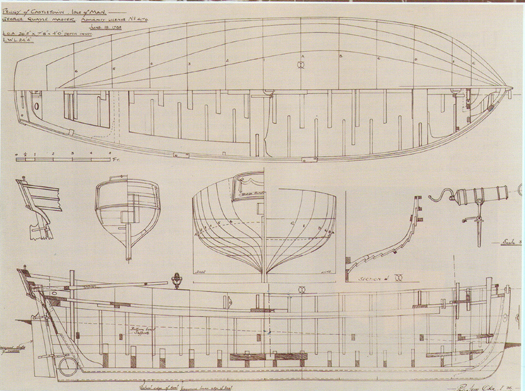
\includegraphics[keepaspectratio]{images/peggy08.jpg}}

}

\caption{Like most craft of her time, Peggy had a full bow and narrow
stern -- the so-called ``cod's head and mackeral's tail'' shape.
Boatbuilders of the time placed great emphasis on having fine lines at
the stern to reduce drag. The full and very buoyant bows were used to
allow the heavy boats of the day to lift their bows over the steep and
choppy waves around England. As warship designer and historian DK Brown
notes, craft of the day also had poor longitudinal structural stiffness,
so heavy weights (like anchors in the bow) had to be supported by
flotation directly underneath, to stop the hull from bending. Compared
to many other boats of her day, though, Peggy's lines seem narrow by the
standards of her day. Although her bows are bluff at gunwale level, they
are quite fine down at water level. Note the tiny cannon that Peggy
carried to ward of privateers (and perhaps other smugglers). That's one
way to ensure you get buoy room!}

\end{figure}%

Quayle had no such problems with his little schooner, which had
centreboards of iron plate. After receiving the challenge from Curwen,
Quayle mounted the tiny swivel cannons that a gentleman's toy needed to
survive in an Irish Sea where French privateers were still active, and
headed across the Irish Sea with two other Manx boats. They sailed up
the River Crake and were placed on carriages for the five mile overland
trip to Windermere.

With her centreboards and her big rig, Peggy swept the opposition off
the lake. ``The Long Bolsprit \& Sliding Keels has already produced
strong Symptoms of Seizure among the Devotees of Fresh Water sailing''
\href{https://sailcraftblog.wordpress.com/wp-content/uploads/2016/05/14733-ms02414-c-obv.jpg}{he
wrote proudly home}. One of the other Manx boats, he noted, was ``the
Second Best in the Lake. Modesty prevents my saying who bears the
Bill.'' \footnote{A letter written by Quayle from London in August 1795
  (MS 02414 Cin the Manx National Archives) indicates that there was at
  least one other boat with three sliding keels under construction in
  the area. One of these may have been the centreboard yachts owned by
  the Commodore of the Cumberland Fleet, the first modern sailing club.}
Peggy kept on racing and winning on Windermere until September had set
in. Even on the stormy trip home, Peggy's iron sliding keels allowed her
to beat home through a gale higher and faster than other Manx boats.
``It can only be imputed to the sliding keels that took advantage''
wrote Quayle.

There had, of course, been other small-boat races before the clash on
Windermere, and the boats of Quayle and Curwen were not what we would
call a dinghy today. But the Windermere race of 1796 remains significant
-- not only is it the earliest small-boat event that we have significant
information about, but it may have been the first race for an open
centreboard craft.

\begin{figure}[H]

{\centering \pandocbounded{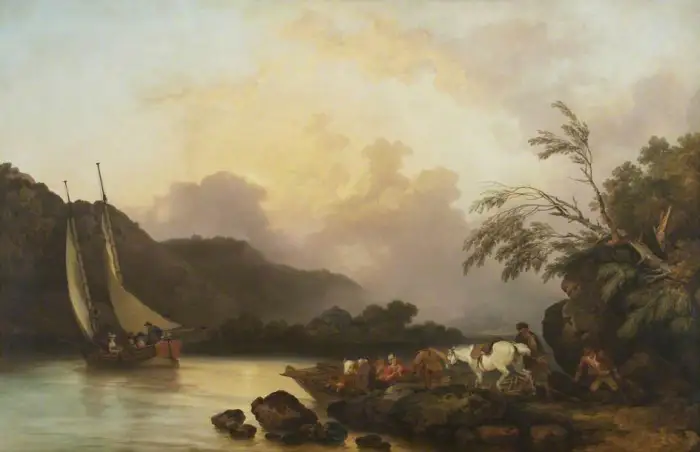
\includegraphics[keepaspectratio]{images/belle.png}}

}

\caption{A small schooner sails past Belle Isle in the late 1700s. The
boat pictured in ``Belle isle Windermere in a calm'' by Philip James de
Loutherbourg could almost have been Peggy, but this picture was painted
in 1786, ten years too early. The painting was bought by John Christian
Curwen, who seems to been a patron of the arts as well as having all the
other marks of a Renaissance man. Photo from the Lakeland Arts Trust.}

\end{figure}%

Curwen kept on running regattas on Windermere after Quayle and Peggy
left; the poet Robert Southey's complaint about the food he arranged one
year is probably the earliest known whinge about regatta catering. One
of Curwen's neighbours, the famous journalist and professor John Wilson,
became a fanatical sailor and owner of a fleet of racing boats, run by
an old sailor called Billy. Like Curwen's biography and Quayle's
letters, Wilson's writing under the name of Christopher North gives us
another glimpse of men whose daily concerns were archaic, but whose love
for the sport sounds modern; ``seldom rose we \ldots{} till, about
twelve o'clock, we heard the south breeze come pushing up from the sea''
he wrote. ``Then Billy used to tap at our door, with his tarry paw, and
whisper, `Master, Peggs is ready. I have brailed up the foresail; her
jigger sits as straight as the Knave of Clubs, and we have ballasted
with sand-bags. We'se beat the Liverpoolean to-day, Master,' Then I
rose.'' He also writes of the pain of being out-pointed ``in our old
schooner, one day when the Victory, on the same tack, shot by us to
windward like a salmon.''

He won the regatta of 1813 with a boat that had the first iron keel on
the lake; earlier boats commonly used stones for ballast.\footnote{The
  Worthies of Cumberland'' Vol 1, Henry Lonsdale MD, 1867.} Quayle, too,
kept on sailing and developing Peggy. After the rough trip back to the
Isle of Man (when one of the other Manx skippers was reduced to bailing
with his wig box) he raised her topsides.\footnote{Details from Nixon, p
  20, and the Friends of the Manx National Heritage website.} Like
dinghy sailors of today, he seems to have fretted when work kept him
from sailing; on 26 June 1803 he wrote to his brother `` `I have had no
Time to get the Boat down yet but have been kept as busy a {[}Trap
Wive{]} in the B {[}ank{]}'. Millions of dinghy sailors have echoed his
complaint since that day. He kept up his interest in centreboards,
meeting and corresponding with Schank and rejoicing when the inventor
praised his understanding of the concept.\footnote{Manx National
  Archives, reference MS 02415 C. Further references to meetings with
  Schank are in MS 02421 C. ``It can only be imputed to the sliding
  keels that took advantage'':- Manx National Archives, reference MS
  00940/5 C. In this passage Quayle referred to the sliding keels'
  assisting Peggy against a tide, which is rather confusing. ``I hope
  left room enough for the little one to lay comfortable'':- Manx
  National Archives, reference MS 00940/3 C.}

The ever-inventive Quayle kept Peggy in a custom-made boathouse, full of
his inventions, in the tiny harbour of Douglas. He seems to have been
forever tinkering with the boathouse; as his brother wrote to him in
1791, ``I hope you left room enough for the little one to lay
comfortable''. Towards the end of his life, Quayle entombed Peggy inside
her custom-made boatshed in the tiny harbour of Douglas. Over time, the
boathouse was walled up and the tiny dock outside was filled in. There
the ``little one'' was to ``lay comfortable'' for decades. In 1820,
Curwen got sick of losing races to his new neighbour, and he left
Margaret to rot.

But that was not the end of the story for Peggy and Margaret. In 1935,
the walls around Peggy's little berth were torn down to reveal that
Peggy and her gear still stood there, complete down to drinking cups
made of coconuts and in astonishingly good condition. Even the bills for
her construction remain in the Manx National Archives, complete down to
details such as the cost of ``halliards'', tar brushes and the weekly
pay sheets, topped by ``Thomas Kelly'' and a boy.

\begin{figure}[H]

{\centering \pandocbounded{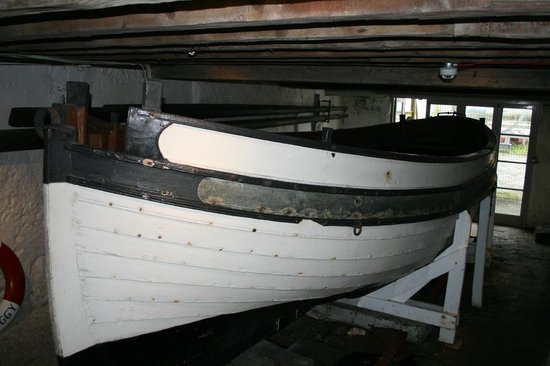
\includegraphics[keepaspectratio]{images/nautical-museum.jpg}}

}

\caption{Peggy, damp but snug inside the boathouse where she stayed for
over two centuries.}

\end{figure}%

Remarkably, Peggy was not the sole survivor of the Winderemere regatta
of 1796. In 1952, G.H. Pattison of the Windermere Steamboat Museum found
the boat that is believed to be Margaret being used as a chicken shed in
the town of Southport. And so, amazingly, the two leading ladies of the
very first recorded centreboarder regatta can still be seen today.

\begin{figure}[H]

{\centering \pandocbounded{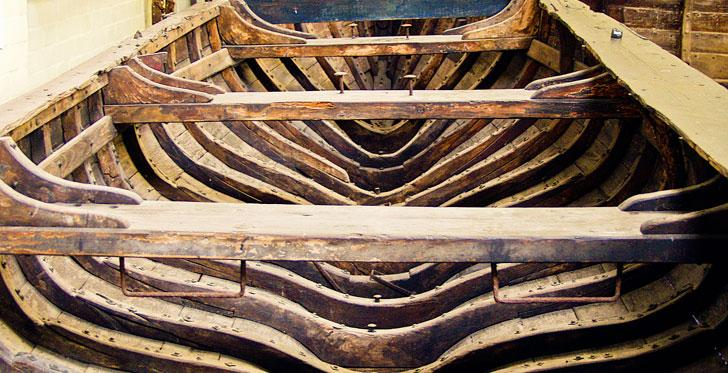
\includegraphics[keepaspectratio]{images/wsm-margaret-header.jpg}}

}

\caption{The hull that is believed to be John Christian Curwen's
Margaret, built in nearby Whitehaven in 1780. Photograph from
\href{https://www.lakelandarts.org.uk}{Lakeland Arts}}

\end{figure}%

\begin{figure}[H]

{\centering \pandocbounded{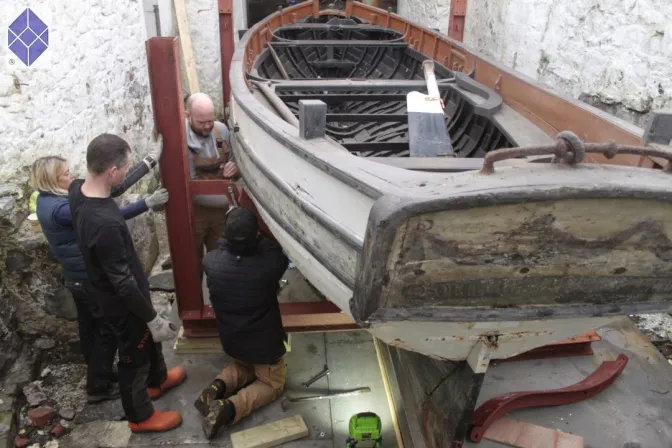
\includegraphics[keepaspectratio]{images/peggy2.png}}

}

\caption{Peggy's construction looks lighter and more efficient than that
of Curwen's Margaret and other boats of her day. The red painted timber
around the gunwales appear to be the extra planks that were fitted to
raise her freeboard after the rough return from racing on Windermere.
Pic from the Peggy of Castletown blogspot.}

\end{figure}%

Margaret is little more than a bare shell \footnote{Details of Margaret
  were taken from WM Nixon's article ``Meetings with Mature Ladies'',
  Wooden Boat, May/June 1986, p 21.} but Peggy is almost complete; still
bearing her 18th century paint and fittings. Today, Peggy is in the
middle of a painstaking long-term restoration project. After six years
of planning and preparation, in 2015 she was gently lifted out of the
boatshed in which she spent two centuries and taken to a preservation
facility. The slow story of Peggy's meticulous restoration can be seen
at \href{http://peggy-of-castletown.blogspot.com.au/}{Peggy of
Castletown}

\begin{figure}[H]

{\centering \pandocbounded{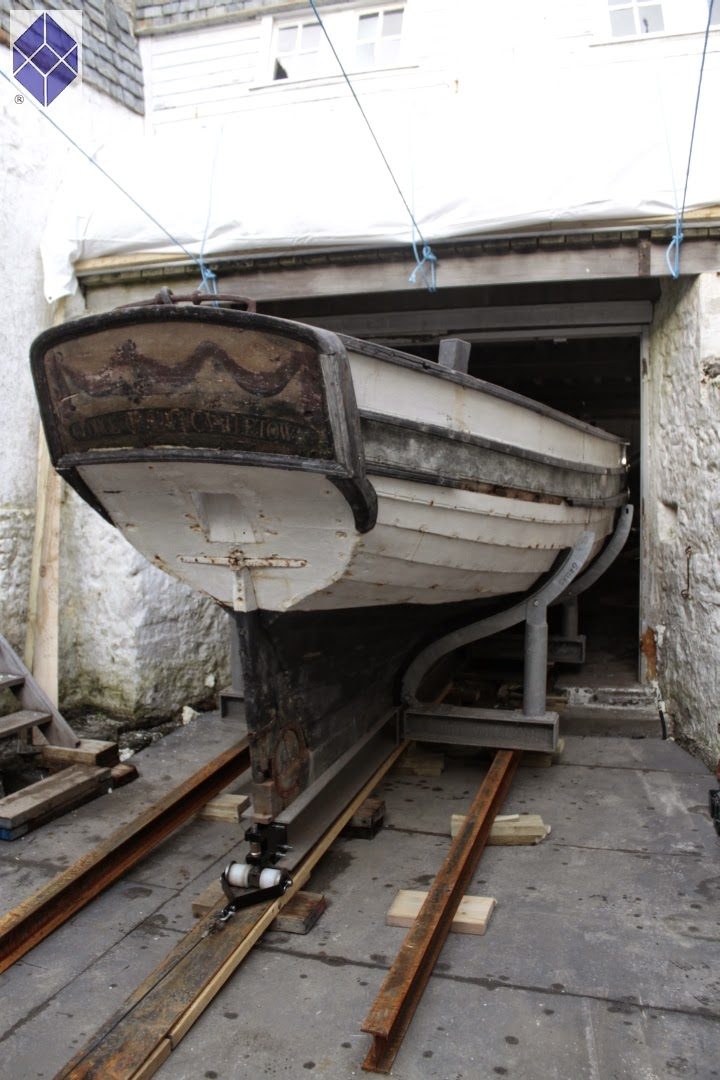
\includegraphics[keepaspectratio]{images/peggy2removal.jpg}}

}

\caption{After over 200 years, Peggy is inched out of her boatshed. Pic
from the Peggy of Castletown blogspot.}

\end{figure}%

But the race on Windermere seems to have been a false dawn as far as
open centreboarders went. The racing sailors of the era stayed with
faithful to long fixed keels and fully decked yachts. One or two
centreboarders raced with the Thames' Cumberland fleet in this period,
but they were fully-decked yachts, complete with full decks and cabins
-- nothing like a dinghy.\footnote{These seem to have included the
  fourth boat christened Cumberland and owned by the Commodore of the
  Cumberland Fleet, the first sailboat racing club. So far I have been
  unable to track down a date for her launch, but it appears that she
  was launched after Peggy's race on Windermere.} The open centreboard
racing boat seems to have been buried for half a century with Peggy.
When it was revived, it was an ocean away.

The men who kickstarted centreboarder racing around 1850 probably never
heard of Peggy. But even after she had been entombed in her boathouse
for four decades, the little schooner's influence may have played a part
in taking the centreboarder all the way to the other side of the world.
\href{https://sailcraftblog.wordpress.com/2016/05/19/sailcraft/}{And
that's another story, for another post}.

\bookmarksetup{startatroot}

\chapter{``Truly as fast as the wind'': Catboats and skimming
dishes}\label{truly-as-fast-as-the-wind-catboats-and-skimming-dishes}

While Peggy slept in her boatshed and Margaret rotted by the lake, the
next ancestor of the modern racing dinghy started to evolve across the
Atlantic. Some time before 1850, when the waters of north-eastern USA
developed the beamy, shallow type that was to become the catboat and the
sandbagger.

The ancestry of the catboat is a mystery. The Dutch, the developers of
the fore-and-aft rig and the first European settlers around the New York
area, had used similar short and beamy boats with a mast stepped well
forward for many years, and some of that tradition may have remained in
the small boats using for fishing, oystering and other work around the
north-eastern USA. But even to authorities like Howard Chappelle and
William Picard Stephens, the greatest of all racing sailboat historians,
exactly when and where the breed developed remained unknown.\footnote{See
  ``Fore \& Aft Craft and their story'', E Keble Chatterton, p 261 and
  305.}

One of the earliest descriptions of the type that for some unknown
reason became labelled the catboat can be found in the recollections of
the legendary yacht designer Nat Herreshoff, who sailed the ``Point
Boats'' that had evolved around the point of Newport Rhode Island by the
mid 1800s. ``Most boats in those days were roughly the type of the old
Julia'' he wrote to his son Francis, referring to a long-keeled boat
approximately 23' long that was built by Nat's father Charles around
1833.\footnote{Capt.~Nat Herreshoff, the Wizard of Bristol by L Francis
  Herreshoff, p39} ``They were nearly all cat rigged with high narrow
sails. In their regattas there were no restrictions as to req. ballast,
so it was the custom to take out part of the standing ballast and
replace it with sand bags and men.''\footnote{This information comes
  from Nat Herreshoff's recollections of his grandfather's tales of
  early sailing, as described to his son L Francis Herreshoff in a
  letter of 10 Feb 1926. Reference: Mystic Seaport Museum.}

\begin{figure}[H]

{\centering \pandocbounded{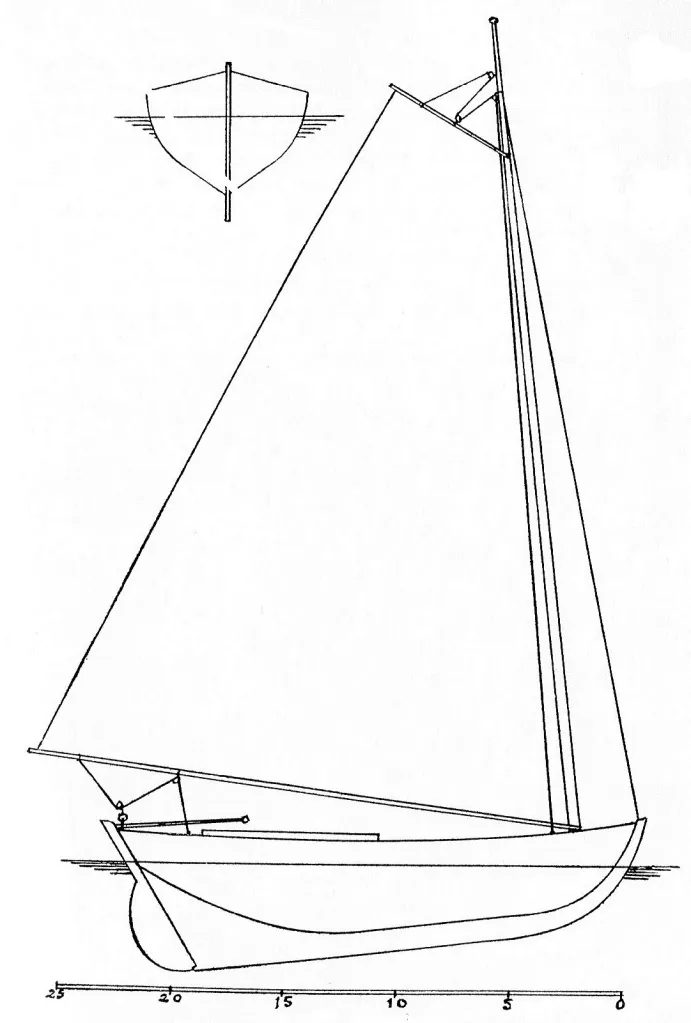
\includegraphics[keepaspectratio]{images/chapter2/point-boat-2.jpg}}

}

\caption{A Newport Rhode Island ``Point Boat'' from the 1830s. This
sketch, reproduced in Traditions and Memories of American Yachting,
shows a boat 23'6″ overall, 7'9″ in beam, and with a draft of 4'9″. The
Herreshoff's Julia was generally similar, at least in profile.}

\end{figure}%

A correspondent in the New York Clipper paper New York Clipper of
November 11, 1854 claimed that ``as far back as 1810,'' he had ``a
beautiful little schooner-rigged centreboard sail boat, with
which\ldots.he used to go forth and outsail everything of her size that
floated: and about the same time, Fountain and Hatfield, of Whitehall,
rigged centreboards to their piraguss, which so improved their working
and sailing qualities that nothing could sail with them.'' \footnote{The
  pivoting centreboard, as distinct from the daggerboard-type ``sliding
  keel'' of Peggy and Schank, was designed by another Royal Navy
  officer, Captain Molyneux Shuldam, when he was a prisoner during the
  Napoleonic Wars. A parallel but slightly later development was awarded
  a patent in the US. Shuldham, described by an Admiral as ``a very
  clever officer'', designed a ``revolving rig'' similar to that of the
  current superyacht Maltese Falcon, as well as a ``harpoon rudder''
  that seems to have been the first spade rudder; Transactions of the
  Royal Institution of Naval Architects, Vol 9 1868 p 273.}

Craft like the ``Point Boats'' remained popular in the deep waters
around Boston and Newport, but in the mid 1800s a different style
started to develop around Cape Cod and in the shallower waters around
Long Island, New York, New Jersey and Barnegat Bay. As Nat Herreshoff
recalled, about 1853 or 1854, ``the cat boats were changing to
centreboard and greater beam, and their rig not so high \& narrow.''
\footnote{Letter of Nat Herreshoff, Mystic Seaport Museum, Feb 10 1926}

The style that is now the archetypal catboat didn't evolve until about
1850, when the Crosby family of Cape Cod launched the first of the 3500
``Cape Cod cats'' they have built. The Crosby cats were heavy
centreboarders, with the mast stepped right in the eyes of the boat, a
hull almost half as wide as it was long, and a huge transom. \footnote{Francis
  Herreshoff believes that the Crosby Cape Cod type was merely one
  example of the catboat's spread up and down the coast, but that ``they
  came into vogue around on Cape Cod where the centreboard cats were so
  popular that many people speak of them as Cape Code cats.'' The
  Compleat Cruiser, p 299} Although the Cape Cod Cat is seen as the
classic catboat today, in the 1800s many localities developed local
breeds. They all used the catboat trademarks of wide, shoal-draft hull
and low aspect rig, but tailored the style for their own conditions and
use.

\pandocbounded{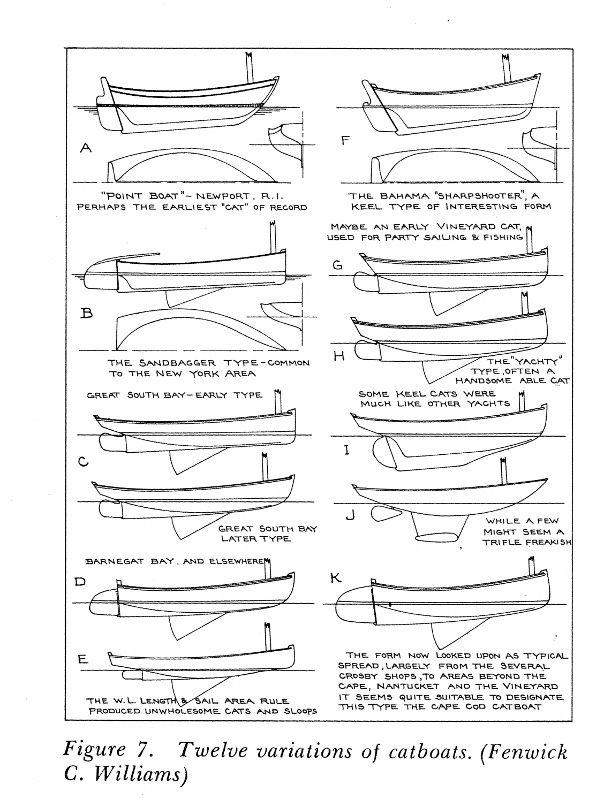
\includegraphics[keepaspectratio]{images/chapter2/catboatvariations.jpg}}

\begin{figure}[H]

{\centering \pandocbounded{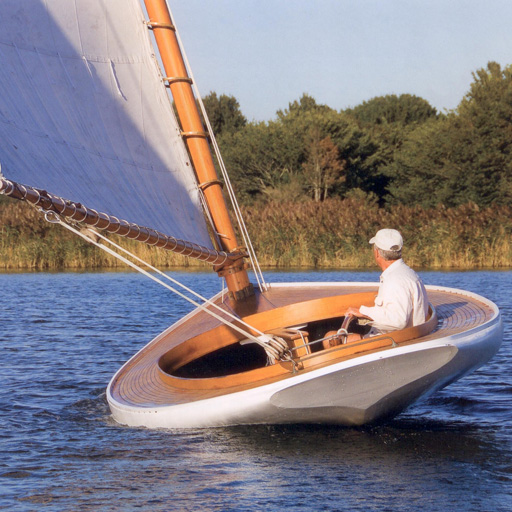
\includegraphics[keepaspectratio]{images/chapter2/gilbertsmith1.jpg}}

}

\caption{Catboats ranged from the elegance of a Gil Smith South Bay
racer to the power of a sloop-rigged Crosby Cape Cod cat. Pics from
Wooden Boat Magazine (top) and catboatforsaleblogspot.com.au}

\end{figure}%

\pandocbounded{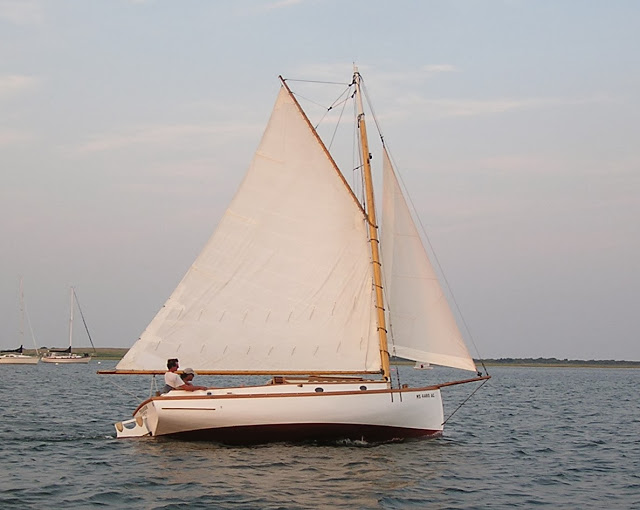
\includegraphics[keepaspectratio]{images/chapter2/teaserundersail.jpg}}

No matter what local breed they were, the 19th century catboats often
carried a bowsprit and jib, especially for racing or the light winds of
summer. A sloop-rigged catboat seems a contradiction in terms today, but
they used words differently in the 1800s. Words like ``catboat'' or
``cutter'', which we used to describe a type of rig, were then used as
the label for a general type of hull. As Nat Herreshoff's brother Lewis
wrote, ``the cat-boat in the usual acceptation means something more than
its simple rig; it stands for a shallow, wide boat, with one mast
crowded into the extreme bow, and a boom reaching far over the stern.''
In typical sailing fashion, just to confuse the uninitiated the sailors
of the time also used the term ``cat rigged'' to refer to boats that
only hoisted a mainsail.

This evolution towards a broad, shallow centreboarder was common around
many parts of the USA. At the start of the 19th century, the waters
around New York had been populated with wide and beamy centreboarders
like the big North River sloops, 75 to 100 feet long, that worked
freight and passengers up and down the Hudson. Fastest of them all was
the giant racing sloop Maria, which had a full 26'6'' beam on a
waterline length of 92' and a draft of just over 5 feet with her seven
ton centreboard up. She was built in 1846 for John C Stevens, founder of
the New York Yacht Club, and easily defeated the yacht America in trials
before the famous schooner went to England and won what would become the
America's Cup. About half the big yachts of New York followed the same
beamy centreboard theme as Magic.

To British yachtsmen, the shallow, beamy American centreboarders were to
become known as ``skimming dishes'' or ``surface sailing'' boats,
because they were thought to skim over the surface of the water, rather
than knife through it like the deep British craft or the pilot schooner
types like America herself. By the time of the first America's Cup
challenge in 1870, the beamy centreboard ``skimming dish'' hull was
established as the American national type, from the smallest catboat to
the largest schooner.

Like many of the big yachts, the small catboats were normally designed
and built by self-taught men, not by trained shipwrights or designers.
``Phil'' Elsworth was an oysterman, Jake Schmidt a hatter and
saloonkeeper. They designed by carving models in pine, and then cutting
them apart to use as the pattern for the full-size boat. Their
experience and innate ability allowed them to create boats that for many
years equalled those of the trained designers.\footnote{See for instance
  ``Traditions and Memories of American yachting'' MotorBoating August
  1944 p 49.} \footnote{``The history of small yacht design Part II'' by
  Russell Clark p 29, Wooden Boat July/August 1981 has information on
  some of the odd thoughts of the ``Rule of thumb'' school.}

One of the greatest of these ``modellers'' was Bob Fish. Born into a
distinguished family, he had been forced to support his family and
siblings when his father died early. ``He was a man of no technical
education, but a born boat sailor, an original thinker, and a very
clever mechanic'' wrote WP Stephens. Lewis Herreshoff, brother of the
famous Nat, rated Fish as second only to Steers (designer of the
schooner America) in his time. Another who ranked Fish highly was A Cary
Smith, who served an apprenticeship in his Pamrope boatshed before
becoming famous for designing America's Cup winners. \footnote{Fish also
  built boats for the Duke of Wellington and worked for Stevens, founder
  of the NYYC and the syndicate that built the schooner America, and as
  the modeller for the NYYC (Brooklyn Daily Eagle 27 June 1889 p 6). As
  expert skipper as well as a builder, like other catboat sailors he
  seems to have turned to a career as a professional racing skipper in
  big boats later in life.}

\begin{figure}[H]

{\centering \pandocbounded{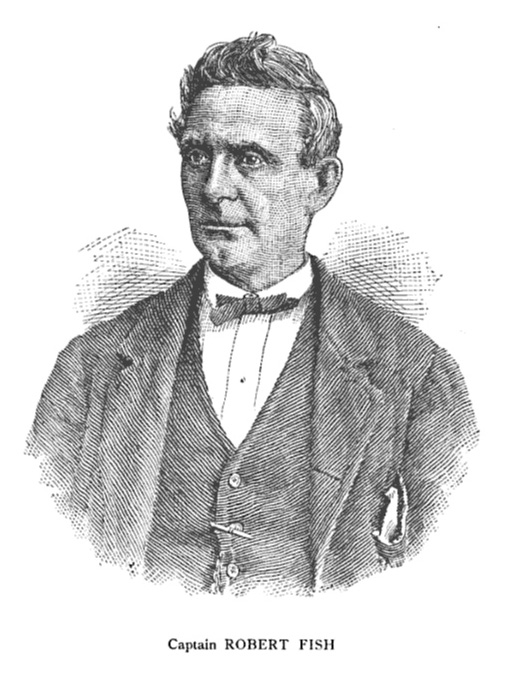
\includegraphics[keepaspectratio]{images/chapter2/bob-fish.jpg}}

}

\caption{Robert Fish -- creator of two of the world's most influential
centreboarders.}

\end{figure}%

It was two of Bob Fish's creations that made the catboat and the
sandbagger famous around the sailing world, even before they were fully
developed in their own home waters. Although the tale of these two
little boats seems to be a diversion from the development of the catboat
type in its American home, it is a tale worth telling because the
sensation they made in England makes them the first well-documented
examples of their type, and also provides an illustration of their
strengths and weaknesses.

In 1852, Robert Minturn Grinnell ordered a jib-and-main boat from Fish.
The two men were linked by their families, which had been partners in
the prosperous shipping firm that had just launched Flying Cloud, one of
the greatest of the clipper ships. Although he was a member of the New
York Yacht Club, Grinnell was about to leave his home town to take up
business in Liverpool. In 1852, little Truant, about 20'/6m overall and
7'/2.1m in beam was delivered to Liverpool, then the world's busiest
port.

\begin{figure}[H]

{\centering \pandocbounded{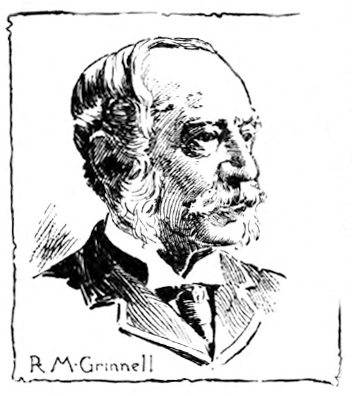
\includegraphics[keepaspectratio]{images/chapter2/robert-m-grinnell1.jpg}}

}

\caption{Robert Minturn Grinnell; the first and most successful skipper
of Truant.}

\end{figure}%

While the Americans had been developing the beamy centreboarder, British
yachting had developed the narrow deep keel cutter. Just as the word
``catboat'' then referred more to a hull shape than a rig, in 1850 the
term ``cutter'' did not simply mean a single-masted boat with more than
one headsail, as it does today. To sailors of the 19th century, it meant
a boat with a deep slender hull (a product of harbour taxation laws,
rating rules and the belief that a narrow boat performed better in
choppy English seas) and a complex rig with a large topsail and several
headsails set from a reefing (retractable) bowsprit. Even small fishing
craft, skiffs and dinghies under 20 feet tended to have complicated rigs
with lugsails or spritsails, jibs and even mizzens. Such rigs may seem
clumsy to our eyes, but they were comparatively easy to reef or douse in
the changeable and often blustery British winds.

The men who sailed the English cutters were far from the modern cliché
of the conservative Victorian-era British yachtsman. Sailboat racing as
an organised sport was young -- little older than the 505 class is today
-- and it was proud to call itself the most progressive and scientific
pastime of the era. Even an ``establishment'' club like the Royal Yacht
Squadron was led by a man (C.R.M. Talbot) who earned his fortune in the
new industries of steel and steam and counted among its members like
Robert Stephenson, creator of the famous `Rocket' steam engine and one
of the new breed of engineers who was transforming the entire world with
railways. Other members included the great Radical journalist Albany
Fonblanque and Joseph Weld, who had created an entire lake on his estate
as a giant test tank. \footnote{Talbot was vice commodore; the commodore
  was the Prince of Wales?} Even those who had the most conservative
political and social views were fascinated by new yacht designs; the
Marquis of Coyningham, pilloried by The Times as one of the worst of the
landlords who lorded over the oppressed Irish in the leadup to the
Famine, was one of those who tried to buy the schooner America. Men like
this and their professional skippers and crews sailed hard, gambled hard
on their races, and were not above fighting with marlinspikes or using
cutlasses and axes to cut a rival's rigging after collisions.\footnote{The
  \emph{Times} of 23 July 1795 reported a collision between Mercury and
  Vixen, in which the captain of Vixen dismantled his rival's rigging
  with a cutlass. See also The New Sporting Magazine, Volume 11 p 181.
  In the Town Cup at Cowes in 1826 a Sir James Jordan allegedly floored
  a crewmember of Weld's Arrow who had tried to bash him over the head
  with a marlinspike after a collision. Rudder v 21 1909 p 11} At least
that was a fair contest; \footnote{See ``Fore \& Aft Craft and their
  story'', E Keble Chatterton, p 261 and 305.} other ``sportsmen'' of
the era got their kicks by watching their greyhounds tear live hares
apart, or shooting hundreds of captive pigeons in a single match.

The big boat sailors of the time believed that they had a duty to use
some of their wealth improve the breed of sailing craft. Sailing was not
just a sport; it was the usual method of transportation for amateur and
professional fishermen, daytripping tourists, and merchant and naval
seaman.\footnote{There was some justification for this belief; in both
  England and the UK , and the brig-rigged yacht Waterwitch beat naval
  ships so often that the Royal navy bought her for a trial horse.}
Until the more economical compound steam engine was developed in the
1870s, even the most modern ironclad warships relied on sail power for
long passages. As one newspaper noted ``the celebrated tea clippers,
which used to make such wonderful passages to England from the China
ports, were the fruits of theory and practice combined and developed in
yacht building.''\footnote{\emph{The Australasian}, 9 July 1881 p3}
Oyster fishermen of the Chesapeake later improved their boats after
reading magazine updates on yacht design, and at least one yachtsman
used to sell his old boats to the local fishermen each year to improve
their fleet. \footnote{Chappelle}

Truant crossed the Atlantic while British yachting was still in shock
from the victory of the schooner America the year before. \footnote{America's
  victory was not won against the best yachts in England. As WP
  Stephens, the leading authority in yachting history of the time wrote
  in his journal. One of the best British yachts lost her and another of
  the top boats went to her aid. The cutter , was only behind the ton
  American schooner at the finish and would have won under any
  reasonable rating or handicap system. America's only other win was
  against Robert Stephenson's Titania, a schooner of half America's
  rated size.} ``The first effect of the visit of the America was
visible in 1851 in the remodelling of the entire British yacht fleet''
wrote WP Stephens. \footnote{American yachting p 71} The big cutters and
giant schooners were being cut down and re-shaped; their bows extended
and made finer. Their full sails were being replaced by flat ones, laced
to the boom. ``The `America' was truly the harbinger of a mania for
clipper-yachts'' said one writer. ``Every yacht and boat-builder
immediately had their hands full\ldots.Such was the complete revolution
in yacht-building created by the performance of that vessel, that more
than half the whole fleet of yachts were altered at the bows\ldots.so
great was the rage to excel and to possess a clipper yacht, that
experiment upon experiment was made.''\footnote{``Yachting and yacht
  racing'', New Sporting Magazine, July 1866 p 21. ``\,''a school of
  marine architecture''; Hunts Universal Yacht List, 1852, p 63.}

Grinnell couldn't have arrived at a better place and time. The sailors
of the River Mersey cities of Liverpool and Birkenhead were just as keen
on development as those who sailed the giant schooners and cutters of
the Thames estuary and the Solent. They included men like members of the
famous Laird shipbuilding family, who had recently launched the world's
first iron warship, complete with ``sliding keels''. Shortly before
America and Truant crossed the Atlantic, yachtsmen of the Mersey
established the Birkenhead Model Yacht Club as ``a school of marine
architecture'' with the aim of ``scientific experiment and practical
deduction'' to improve boat design. To the BMYC members, the word
``model'' had three meanings. As well as the obvious meaning of scale
model, it was also a common term for the physical shape of a yacht's
hull at the time. Finally, and perhaps most importantly, there was the
connotation of ``an example to follow or imitate'', as in the term
``model of perfection.''

The men who formed the BMYC, once called ``the mother of small yacht
clubs'', ranged from titled big-boat owners to immigrant students, but
they were united by a desire for a ``progressive and scientific yacht
club'' that would improve boat design by testing models.\footnote{The
  Australian Town and Country Journal, 5 May 1888 p 39; Ballarat Courier
  7 Sep 1877} ``5000 persons assembled to witness the match. I will
never forget the sight as long as I live'' remembered one witness to one
of their model yacht races in the docks near Liverpool ``up to nearly
their waists in the water stood some 15 gentlemen, including\ldots a
well known medico\ldots.and one of the young Lairds, who then owned a
yacht of some 35 tons.''\footnote{Bell's Life in London and Sporting
  Chronicle, June 20, 1852. The report says that she was normally cat
  rigged, but it appears that when racing she normally carried a jib.}

Some BMYC members quickly found out that the choppy water of the dock
and the effects of scale meant that their tests were misleading, and
decided to continue their experiments with full size boats. ``Owing to
the dissatisfaction of several of the more progressive spirits at the
results of our model experiments, craft of from 4,5,6,7 and 8 tons were
at once built'' foundation member H.R. Murray recalled years later.
``And no sooner did they spread their white wings over the Mersey than
(a ship) brought over a queer-looking centreboard craft'' wrote Murray.
\footnote{Ballarat Courier, 7 Sep 1877}

\begin{figure}[H]

{\centering \pandocbounded{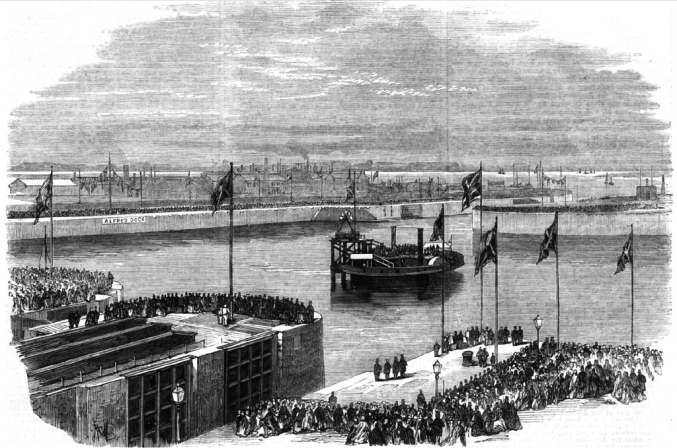
\includegraphics[keepaspectratio]{images/chapter2/birkenhead.jpg}}

}

\caption{Birkenhead's ``Great Float'' dock, dressed for its official
opening. Titled and wealthy men with a passion for boat design used to
race model yachts in this unlikely industrial setting.}

\end{figure}%

The ``queer craft'' was Truant. The little American boat caused a
sensation. She was ``another America; dissimilar in some respects, but
greater as developing a great novelty'' raved one paper. ``Her
peculiarity consists not only in her rig, but in her hull'' which was
``about as flat as a butchers tray, sharp in front but full behind. She
has a shifting keel by which she can either draw about eight inches of
water only when running, or about 4'6'' when beating, at which time only
her keel is put down like an ordinary boat's. Of her rig next. She has
her mainsail flat as a board and laced; and carried forward what is
known to yachtsmen by the appellation of a ``bumpkin'' foresail, also
laced to the boom. These, with a small topsail, constitute her suit: and
a smarter suit it would be difficult to find\ldots{}\footnote{The Era,
  May 22 1853}

The ``strange-looking little foreigner\ldots has her mast stepped in her
very eyes- has a long easy entrance -- full withal, and not a hollow
line about her -- carries her body all aft -- does not draw much more
water than about a foot in ballast trim -- sails with a small centre
board'' noted another fascinated reporter. ``She is about twenty feet
over all, and seven feet beam.''

Unlike the British cutters, Truant could sail well under mainsail alone,
although she did sometimes set a topsail. When racing she appears to
have normally carried a jib set on a boom which (like the rig of a
modern model yacht) pivoted on a point aft of the tack.

\pandocbounded{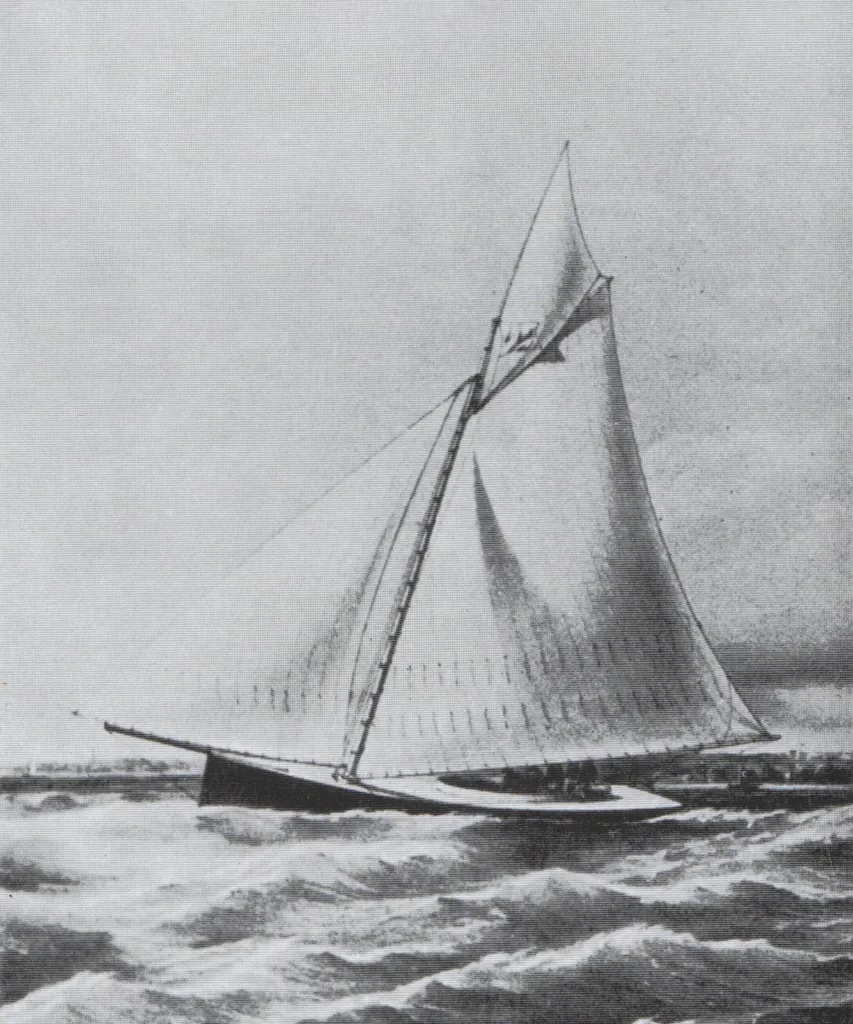
\includegraphics[keepaspectratio]{images/chapter2/truant.jpg}}
Even before her first race, Truant's performance on the narrow Mersey
River amazed the locals. ``Truly she is as fast as the wind -- staying,
wearing, running and reaching under the single sail with amazing
velocity'' one journalist reported. \footnote{Bell's Life in London and
  Sporting Chronicle, June 20, 1852. The report says that she was
  normally cat rigged, but it appears that when racing she normally
  carried a jib.} In her first race the little boat, rated at 3 1/2
tons, ``shot away''\footnote{Manchester Times, June 30 1852. Truant
  often raced with Birkenhead Model Yacht Club on the Mersey River at
  Liverpool. Birkenhead, like its London counterpart, used the term
  ``model'' to mean an ideal full-sized boat, not just a ``toy'' or
  miniature one. As noted in Bell's Life of December 19 1852, the club
  ``was formed expressly and entirely with a view to the improvement of
  model'', and so raced full-sized craft of up to 8 tons. The early
  fleet was made up of ``old boats'' converted into yachts, such as
  Alfred Bowyer's Mosquito, but custom-built yachts soon arrived.} to
finish 16 minutes ahead of the fleet. ``Although the Yankee has, on this
occasion, again `whipped all creation' the best feeling was manifested;
and Grinnell was highly complimented by the commodore in awarding to him
the cup.'' \footnote{The Brooklyn Daily Eagle, 14 Aug 1852, p 1}

\begin{figure}[H]

{\centering \pandocbounded{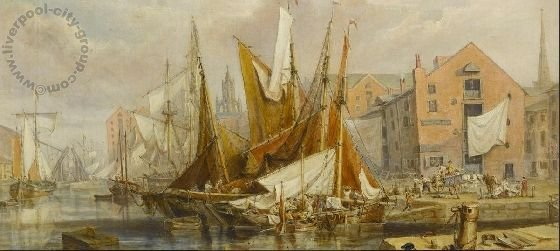
\includegraphics[keepaspectratio]{images/chapter2/liverpool-history-waterfront-1850.jpg}}

}

\caption{Liverpool docks in 1850, when sail still ruled the world's
busiest port, and improving hull designs saved lives and money.}

\end{figure}%

By July, Grinnell had shipped Truant across the Irish Sea, and ``the
Yankee cockleshell'' was amazing the Irish regatta circuit. \footnote{Freeman's
  Journal and Daily Commercial Advertiser, July 21 1852} She could ``go
about in the most extraordinary manner, in fact exactly like a top''
exclaimed the Cork Examiner, and ``gaining ground on every tack'', she
``shot off rapidly'' to win.\footnote{The Cork Examiner, July 28 1852 p
  3} The ``extraordinary little yacht'' was ``now as famous in Dublin
Bay as she had previously become at Liverpool.''\footnote{Hunts Yachting
  Magazine, September 1852, p 105}

Truant gained her most noted success after she was shipped down to the
Thames, site of the world's first organised yacht racing club. The
unbeatable American was already so famous that before the race, Bells
Sporting Life was warning spectators to book early for the spectator
ferry.\footnote{Bell's Life in London and Sporting Chronmicle, 1 May
  1853, p 6} In the race she showed herself to be ``infinitely
superior'' upwind, winning by a quarter of an hour from larger boats
before being ``greeted with loud cheers, which were taken up by several
of the yachtsmen afloat in their own craft.'' \footnote{The Era, May 22,
  1853} Truant's triumphs were not just local news; they were reported
as far afield as New York and Australia.

``The performances of this little vessel in beating to windward and
scudding before the wind were astonishing'' wrote contemporary sailor
Henry Folkard in his enormously popular book Sailing Boats. ``No English
boat her size could sail so close to the wind, nor run so swiftly before
the wind; and the result was, that the Truant completely vanquished on
the river (as her larger sister the America had done on the sea) every
boat that competed with her. \footnote{Folkard p 94}

The New Sporting Magazine compared Truant's impact to the that of the
schooner America. ``No English boat of her size could compete with her;
and thus a second revolution was brought about; and boat-builders
puzzled their brains over this new discovery which now dawned upon them,
as the astonishing performance of this little clipper were from time to
time witnessed in every match she sailed.''\footnote{Yachts and
  yacht-racing'', New Sporting Magazine, July 1866, p 22}

One of the boatbuilders who puzzled over Truant was H.R. Murray of the
BMYC. Years later, he was to use the term ``surface sailing'' to
contrast the American centreboarders with the deep British boats. ``The
hull should skim over the surface of the water, while the immersed blade
increases the lateral resistance, and enables them then in ordinary
weather to hold a wind with their deep-keeled rivals.'' It was a
description that echoed Schank's words of the 1700s, and that Murray
would take across the world. \footnote{The \emph{Times} of 23 July 1795
  reported a collision between Mercury and Vixen, in which the captain
  of Vixen dismantled his rival's rigging with a cutlass. See also The
  New Sporting Magazine, Volume 11 p 181. In the Town Cup at Cowes in
  1826 a Sir James Jordan allegedly floored a crewmember of Weld's Arrow
  who had tried to bash him over the head with a marlinspike after a
  collision. Rudder v 21 1909 p 11}

\pandocbounded{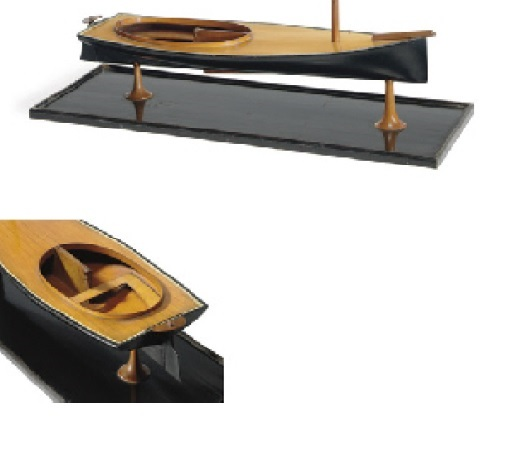
\includegraphics[keepaspectratio]{images/chapter2/truant-model.jpg}}
Although there were some who jeered and even some who cursed, the
available evidence indicates that the overall reaction of the Victorian
yachtsmen to Truant was positive. As early as November 1852, Grinnell
noted that builders from all parts of the UK were copying her model, and
as soon after Truant returned from the Thames to her home waters at
Liverpool, she started facing competition from other boats built along
the lines of the American centreboard sloop. \footnote{Irish Examiner,
  22 November p 2. It is interesting to see that this comment came in an
  advertisement for the boat, although Grinnell himself continued to
  race his larger schooner around Liverpool.} The Mersey fleet soon
included the centreboarder Breeze built along American lines, the 10 ton
Stranger, a keelboat built to the centreboard sloop concept by Bob Fish
himself and carrying up to 12 crew as live ballast, and another Fish
export, the little 2 ½ ton Buffalo Gal that was later sailed by
Grinnell. \footnote{Hunts Yachting Magazine, December 1852, p 291.
  Grinnell raced one of the imported Fish products, the little Buffalo
  Gal, to second in a race at Windemere in spite of being by far the
  smallest boat and facing a ``hurricane'' of a headwind; Hunts 1859 v 8
  p 516.},\footnote{Bells June 12 1853 p 5}

Probably the keenest of all the Mersey centreboarder fans was the cotton
merchant Alfred Bower.\footnote{Bowyer's earlier boat, possibly one of
  the converted open boats that the BMYC started with, had capsized and
  instantly sunk in the Mersey in 1852; Manchester Courier and
  Lancashire General Advertiser (Manchester, England), Saturday,
  September 11, 1852; pg. 7} In his obituary is was noted that Bower
``to his last was a firm believer that, for speed, the centre-board
would beat the deep keel craft hands down.''\footnote{Australian Town
  and Country Journal 5 May 1888 p 39} For several years he had a new 8
ton centreboard sloop type built every year; first Presto, then
Challenge, Charm, Spray, each with 670lb/300kg) of movable ballast
mounted on ``tramlines'' that ran across the cockpit -- an idea that the
legendary Herreshoffs only adopted about a decade later.\footnote{The
  information about the movable ballast in the Bower boats comes from
  classified ads when the boats were put up for sale in the early to mid
  1850s. L Francis Herreshoff says that the second Julia was fitted with
  a similar device in 1864. She had 550 lb of iron ballast mounted on a
  slide that ran on railway tracks across the cockpit Traditions etc,
  MBing Sept 1942 p 52 clled the movable ballast ``unwieldy and
  dangerous'' but Francis quotes Nat (p 41) as saying that there were no
  problems with it and it made Julia (2), not a new boat, the fastest of
  her type in the district.}

Presto, Challenge and Spray were each built by local boatbuilder Philip
Kelly. And here we come to an intriguing note -- for the only
boatbuilder of that name I can identify in the area at the time was in
his late 60s, but still healthy enough to woo and marry his third wife a
few years later. The marriage records show that the ageing Philip Kelly
had been born in Douglas to a shipwright named Thomas Kelly in Douglas
on the isle of Man in 1786. Was this the same Thomas Kelly who was
listed in George Quayle's accounts for the construction of Peggy? Was
the young Philip Kelly the first ever boy to be fascinated by a champion
centreboarder, and to decide to devote his life to building boats? Did
he chuckle when the `new fangled' centreboard, similar to the ones he
may have worked on 50 years before, arrived at his Liverpool home when
he was an old man? It's hard not to think that the Philip Kelly who
built Bower's boats must have grown up on the Isle of Man, watching his
father build Peggy under George Quayle's direction, and perhaps lending
a hand on her modifications in those days when children started their
apprenticeships early.

But despite the enthusiasm for the American centreboard sloop, within a
few years the type seems to have died out. Race reports become once
again a contest of deep, narrow cutter against deep, narrow cutter. So
why did the American centreboard sloop fade out in Britain? In part, it
was due to the fact that the rating systems of the day favoured the
traditional deep and narrow cutter. Truant, 20' long overall, only had a
handicap of a minute per race over Julia, the runner-up in the race on
the Thames, which was more than 30' overall.\footnote{Even traditional
  British types suffered the same way; the Little Mosquito, apparently
  built to the Itchen Ferry's length restriction, was ``beating
  everything in turning to windward'' but was noted to be ``built to
  sail by length, not by tonnage' so rated one ton higher (a minute per
  race) than a boat like Julia which was several foot longer, and
  carrying, at least, a fifth more sail.'' -- Bell's Life in London and
  Sporting Chronicle (London, England), Sunday, July 29, 1855; pg. 8.}
But the rating system itself could not have killed the centreboard
sloop; they could still win races, and other types that rated poorly
(like the Itchen Ferry Punts) did not die out.

The centreboard itself attracted some criticism. Some said that it was
``a dodge'' that allowed her to sail into shallow waters and escape
unfavourable tides. \footnote{One writer, referring to larger boats,
  referred to the centreboarder's ability to `cheat' tides and said that
  if all courses were in deep water, like Kingstown in Ireland,
  centreboards would be allowed -- but as most racing was done in tidal
  rivers, they had too much of an advantage; Hunts Vol 19, 1870 p 554 .
  A BMYC owner who had refused to race his keelboat against the
  centreboarders on the Mersey because he felt they had an unfair
  advantage in tidal waters later bought Truant and raced her with
  success in Kingstown.} Years later one ``establishment'' owner was to
comment that ``for many years there was a curious dislike and distrust
of (centreboards) among British boat-sailers and builders. They were
excluded altogether from most regattas; and not one in twenty of the
boats that would have been vastly improved by them were ever fitted with
them. They were regarded, for some mysterious reason, as unseaworthy,
unsportsmanlike, and unfair.''\footnote{Yacht's Sailing Boats, Earl of
  Pembroke and Montgomery, Yachting vol 1, Badminton library p}; Others
said that the movable centreboards should be banned because they were a
return to the curse of shifting ballast that had blighted British
yachting for years. \footnote{Until a few years before, even the larger
  British boats had carried tons of lead shot in bags, which was dragged
  or tossed to windward each tack. It was a dirty, exhausting and
  unpleasant operation that cost owners dear, both to have their yacht's
  accommodation modified and cleared out before each race, and for extra
  paid crew to replace the amateurs who rebelled against spending their
  leisure hours throwing metal around a tossing hole. At least one
  sailor died when the ballast they were moving fell to leeward and the
  boat sank with him trapped in the cabin; The Sporting Review, Review
  of the yachting Season of 1857 p 248. Around the time of Truant,
  individual clubs and regatta organisers restricted shifting ballast,
  which was eventually banned by the RYA (then the yacht Racing
  Association) in 1875. There were apparently rumours that Truant
  carried movable ballast, and Bower's boats certainly did.} Still
others spoke of leaking centreboard cases, while Francis Herreshoff
noted years later that stones from the British shingle beaches often
jammed 'boards.

Although it is often said that centreboards were banned from British
yachting, in Truant's day there was no national body to enforce such a
ban, and the two major small-yacht clubs, Birkenhead and the Prince of
Wales, either permitted them or, following the standard practice of
grouping boats of similar type into specific classes, ran separate
classes for centreboarders. Some years later, other regatta organisers
and clubs did ban centreboards, and they were specifically banned from
the bigger yachts, but at this distance it is hard to find any evidence
that prejudice or blind conservatism was the reason.

There were those who criticised Truant and similar centreboarders as
nothing more than ``sailing machines''. ``We may just as well call her a
yacht as term a match-cart (i.e.~a horse-racing sulky) a comfortable
family carriage'' said one writer after Truant's victory in the Thames.
\footnote{Hunts Yachting Magazine, Vol 2, 1853, p 151} ``A shallow
skimming dish should hardly be allowed to sail in matches, in which
vessels possessing the usual accommodation were competitors, and almost
certain to be distanced.''\footnote{Hunts Yachting Magazine (?) p 105}

It was, in truth, a fair point. The boat that ran second to Truant on
the Thames was Julia, described as ``a very peculiar model'' of boat,
built in iron to a design by her owner. \footnote{Hunts Yachting
  Magazine, 1857, p 422} Rated at 7 tons, she had a waterline of 26'6''
LWL, a beam of 7'11'' beam, and was about 30 feet long. She was a much
larger boat than Truant, but she also had a 10' long saloon with
standing headroom that would seat half a dozen in comfort. \footnote{Hunts
  Yachting Magazine, Vol 3, 1854, Vol p 506} The Ida, which placed third
that day, was only 22'6'' long but had completed a 20 day cruise to
France.\footnote{Hunts Yachting Magazine and WP Stevens provide
  information on the cruise, while Stevens provided information on Ida's
  dimensions.} Truant, in contrast, was an open day-sailing racer that
was carried from race to race aboard ships.\footnote{See for example,
  Irish Examiner August 2 1852} Even in larger sizes, the centreboarders
had their accommodation cut up by the centreboard case and the deck
obstructed by the large deckhouse required for headroom.\footnote{After
  an early win in Ireland in July 1852 some objected to the fact that
  Truant had boomed out her headsail (as America had been allowed to do)
  and ``a sailor, who had been in the second boat, came up and formally
  cursed her for the loss of the victory -- a duty which he performed
  with entire simplicity and sincerity of feeling.''{[}45{]}} Putting a
boat like Truant up against these seaworthy cruiser/racers was like
putting a skiff in a sportsboat race.

But in the end, the Mersey centreboarders may be an early example of the
fact that weather, society and geography dictate design. The beamy
centreboard sloop often performed brilliantly on the Mersey, Thames and
Dublin Bay, but it may not have suited other British conditions. As the
celebrated yachting writer William Cooper (writing as Vanderdecken)
noted, in flat water, downwind or in steady conditions the American
sloop type was ``admirably adapted, and of wonderful speed'' but they
were inferior in typical English conditions of blustery winds and choppy
seas, cut up by tides and overfalls. ``They are not calculated for our
seas'' was his conclusion\footnote{In the Gaff Rig Handbook, John
  Leather refers to Truant as ``a poor seaboat'' that probably won
  because of her rig, but he gives no source or evidence for these
  remarks. Cooper believed that Grinnell was the only man who could
  really sail the sloop properly, but in fact she won her race on the
  Thames under a guest skipper, and after some bad luck early on she
  also won in Ireland with another hand at the helm. She also returned
  to Grinnell's control by 1856 for at least one race.}.

Cooper`s criticism could perhaps be dismissed as bias or conservatism,
if it was not borne out by so many race results and reports that spoke
of the centreboard sloops retiring or lagging behind deep-keel cutters
in strong and gusty winds and choppy seas. \footnote{Among them, Hunts
  1858 p 260-1; 1858 v 7 p 224; note in this race 3 of the 4 entries
  were centreboarders; the event was won by a 33' cutter.} \footnote{For
  example, Hunts 1870 p 552} Sir William Forwood's story demonstrates
that ``establishment'' figures like him were not scared of the new style
of centreboarder, or ignorant of its problems. He had sailed on several
of the centreboarders owned by his uncle Alfred Bower. In 1866 he bought
Truant ``which had greatly distinguished herself for speed, and taking
her up to Windermere'' he wrote. ``She was not, however, of much use on
that expansive but treacherous sheet of water. The heavy squalls were
too much for her huge sail plan.'' \footnote{``Recollections of a busy
  life'', Sir William B Forwood, 1910, Chapter xix. Forwood went on to
  commercial and political success and was one of the founders of the
  Royal Yachting Association, which appears to demonstrate that the
  centreboarders had support from the ``establishment'', who were not
  always against innovative types. Grinnell was also a powerful man; he
  was not just rich but also had strong support from the press, who
  reminded readers that his father had paid for Polar expeditions in
  search of the lost Royal Navy ships Erebus and Terror.}

\begin{figure}[H]

{\centering \pandocbounded{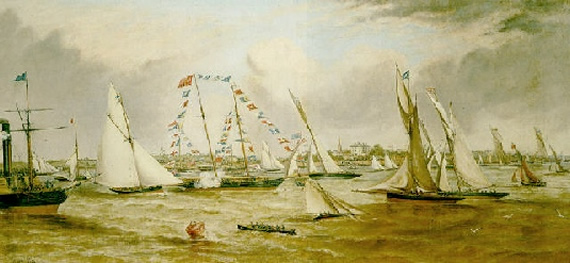
\includegraphics[keepaspectratio]{images/chapter2/coralie.jpg}}

}

\caption{The cutter Coralie (left) takes the winner's gun in a Royal
Mersey Yacht Club race in 1847, five years before Truant arrived in
Liverpool. The big cutter's owner was one of the BMYC members who used
model yachts to test new designs. Coralie was to become one of the
rivals of the bigger Bob Fish and Philip Kelly designs such as Challenge
and Stranger in a series of interesting battles between the deep British
cutter and the shallow American centreboard sloop. This copy of the
Henry Melling painting comes from the RMYC site.}

\end{figure}%

Many years another writer who had learned to sail on the Liverpool
sloops wrote of their ``alluring excitement'' but claimed that sailors
were turned off by their dangerous and uncomfortable performance in the
choppy, windy and cold British conditions. An Australian yachting writer
claimed years later that the Liverpool sailors laughed ``when they
recall to memory their folly, and the risk they used to run in the
useless and unseaworthy boats, which they looked upon at the time as not
to be beaten by anything afloat'' \footnote{Australian Town and Country
  Journal, 1 April 1882 p 32. It should be noted that the un-named
  writer did not provide any evidence for his claims.} Even Truant
herself, sailed by the experienced Grinnell, capsized twice on the
Mersey.\footnote{Bell's Life in London and Sporting Chronicle , November
  25, 1855, p.5.} Anyone who looks at the Mersey could wonder how they
would right and empty a big 19th century centreboarder among those
chilly tide-ripped waters and steep riverbanks.

Truant's career shows a trend that extends to the present day. The fact
that some people disliked the type is seen by some modern commentators
as unfair bias by a blind establishment. In fact, judging from the press
accounts, those who cursed Truant were greatly outnumbered by those who
cheered her.\footnote{See for instance Bell's Life in London and
  Sporting Chronicle, July 25, 1852, p.5, which spoke of the ``wonderful
  little craft\ldots beautifully handled by her open hearted and
  spirited owner.''} Some reports of her performance exaggerated her
record, rather than diminished it. \footnote{``But true to his beliefs,
  Arthur Bower kept his last centreboarder'': -- Australian Town and
  Country Journal, 5 May 1888 p 39.} In the end, it seems that the
American centreboard sloop died out in Britain not because of
establishment bias (although the rating rule was harsh on them) but
because they were unsuitable for cruising and inconsistent and
uncomfortable for racing in English conditions.\footnote{The fact that
  Truant's owner Forwood was one of the founders of the RYA indicates
  that ``the establishment'' had much more experience of the American
  centreboard sloop than later critics.} It might be significant that
when the Mersey developed another local centreboard class in the 1880s,
the class rules created a slender (5'8'' to 6' beam) 18 footer with a
moderate sized 280ft2 rig rather than a beamy American sloop
type.\footnote{A century later, the gaff rig expert John Leather noted
  that one of these 18 Footers, Zinnia, was similar to a sandbagger or
  catboat and mused whether her designer had seen such plans in Dixon
  Kemp's earlier editions. It is more likely that he was aware of the
  Mersey centreboarders that were inspired by Truant. Kemp edition p 354}
But true to his beliefs, Arthur Bower kept his last centreboarder,
Enigma, laid up for 20 years, and to the end of his life he occasionally
brought her out to ``show them how a race should be sailed''.

And what of Grinnell? After selling Truant, he also occasionally raced
his big schooner on the Mersey. When the American Civil War began, this
member of the New York establishment took up arms against his own side
by joining the southern Confederate forces. Remarkably, after the south
lost the war he appears to have returned to New York, but unlike the
rest of his family he dropped out of sailing.

But even as the craze for the American centreboard sloop started to
fade, the model started to spread further afield. Men and boats inspired
by Truant ended up taking the ``surface sailing'' model across to the
far side of the world. Bob Fish himself started to export centreboard
sloops to Germany, especially to the tiny ornamental lake Alster in
Hamburg. Was Fish's export drive spurred by the fact that one skippers
entered against Truant in the famous race on the Thames was a Herr
Westphal from Hamburg? But that is another story, and
\href{https://sailcraftblog.wordpress.com/2016/05/20/sailcraft-pt-3/}{first
we must look at the next Bob Fish boat to cause a sensation
overseas\ldots{}}

\bookmarksetup{startatroot}

\chapter{``A little too marvelous to be real'' -- the story of the Una
Boat}\label{a-little-too-marvelous-to-be-real-the-story-of-the-una-boat}

\bookmarksetup{startatroot}

\chapter{The Sandbaggers}\label{the-sandbaggers}

\bookmarksetup{startatroot}

\chapter{The mysterious history of the
sharpie}\label{the-mysterious-history-of-the-sharpie}

Although the sandbagger and the catboat took most of the attention that
small boats received in the late 1800s, not far away another breed was
developing more quietly. It was the sharpie, and while it didn't bring
the world's attention to the potential of the centreboarder like the
sandbaggers and catboat did, it may have had more direct influence on
the shape of the modern dinghy.

The key word, however, is ``may''. Tracing the history of the sharpie's
influence on dinghy design is a frustrating exercise on many levels. The
working sharpies and their relatives have been the subject of an
intimidating amount of research from people like Howard I Chapelle,
Reuel Parker, and Pete Lesher, but even authorities like Chapelle
admitted that some aspects of the sharpie's history remain murky.
Tracing the influence of the sharpie on racing dinghies poses an even
harder problem. There was no small sharpie that played the starring role
of Rob Roy, Truant or Una, and there was no racing scene like that of
the sandbaggers to catch the attention of researchers and writers.
Reports from some areas hint that the same economy and simplicity that
attracted some racing sailors to the sharpie seem to have led others to
ignore it.

There are big holes in the story of the sharpie, and they will probably
always remain. Even the fact that a boat is called a sharpie may not
show that it has any connection with the American craft -- after all, we
use the Hindi and Tamil words ``dinghy'' and ``catamaran'' for boats
that have no relationship with the Indian craft that originally bore
those names. Flat bottomed hard-chined boats are so obviously simple and
easy to build that they have been seen in many civilisations for
thousands of years. We know that flat-bottomed boats evolved from other
types, such as punts, in several places across the world. Some may
merely have had the ``sharpie'' label stuck onto them retrospectively,
in the same way that some classes that have no ``skiff'' DNA have known
become known as skiffs. Even experts on sharpie design like Chapelle and
Parker believe that some of the American sharpies, like those of the
Chesapeake and Great Lakes, evolved independently. If the sharpie shape
and form could be developed independently in two or three places in the
USA, it's obvious that it could have evolved independently in other
countries as well.

Given all these issues, in some ways it would have been easier to pass
lightly over the early evolution of the sharpie and its influence on
dinghy design, but that would have meant ignoring a significant step in
the story of the racing dinghy. So let's try to see how the sharpie-type
dinghy may have evolved, and hope that further information and research
could make the murky story a bit clearer.

The type that is normally identified as the original sharpie evolved
around the fishing port of New Haven, 110km/70 miles from New York on
the Connecticut shore of Long Island Sound. As in so many other cases,
the sharpie was created by the area's local forests, industry, fisheries
and oceanography. The huge area of shoals of Long Island Sound formed
immense oyster fisheries that were best worked with fast shoal-draft
craft. Originally, the oyster fishermen used huge dugout canoes, from 28
to 35 feet long, that were cut from the vast forests of white pine
around Connecticut and upper New York. Down south on Chesapeake Bay,
fishermen enjoyed similar conditions and adopted similar craft, carving
canoes as long as 30ft/9m from a single log. As the demand for larger
craft grew, the watermen of the Chesapeake began building canoes from as
many as five logs, each bolted together to form giant planks across the
bottom.

\begin{figure}[H]

{\centering \pandocbounded{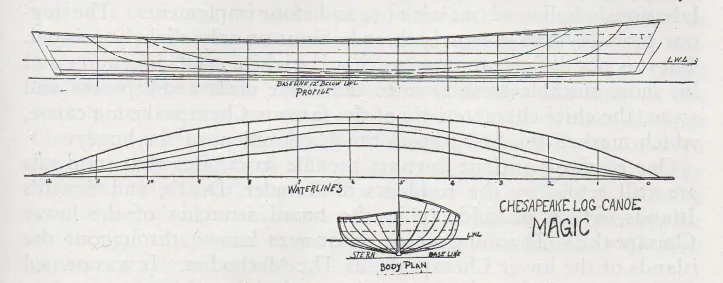
\includegraphics[keepaspectratio]{images/chapter5/sailing-canoe-magic.png}}

}

\caption{The beautiful lines of the 34'/10.4m log canoe Magic, built
from five logs in 1894 and one of the most successful such craft ever
built, gives a glimpse of what the sharpie's ancestors may have looked
line. By the time she was launched, log canoe racing was a serious
sport, and canoes like Magic were being built especially for racing.
Lines from `The bugeye of the Chesapeake' by Peter C Chambliss in the
outstanding book Sailing Craft, edited by Edwin J Schoettle in 1937.}

\end{figure}%

Some time around the mid 1800s, the supply of white pine around New
Haven ran out, and the local oystermen started looking for an
alternative. ``What more natural than that they should have applied to
the nearest sawmill for plank for which to nail up a box in imitation of
the more costly and complicated round-ribbed composition of the regular
boat builder?'' asked Forest and Stream. ``The box was run to a point at
one end, and a single wide plank on the bottom was rounded up aft, as
the nearest approach to regular boat form three planks could be induced
to assume. Simple and cheap, every man became his own builder during the
sawmill era, rip and cross cut supplanting the axe and burning process
of the days when big logs were common.'' And so the sharpie was born.

\begin{figure}[H]

{\centering \pandocbounded{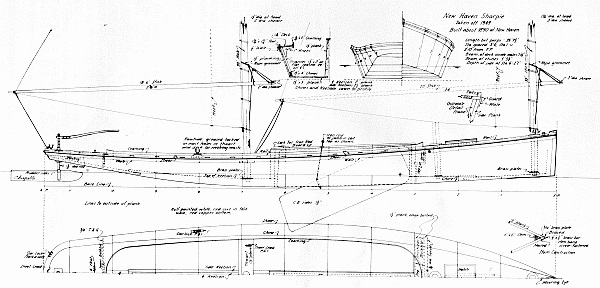
\includegraphics[keepaspectratio]{images/chapter5/sharpie-from-chapelle.jpg}}

}

\caption{A New Haven Sharpie from Chapelle's ``Migration of an American
Boat Type''.}

\end{figure}%

The sharpie followed the log canoe's long, slender shape, and was
normally four or five times as long as it was wide. It also kept the
canoe's simple but heavy construction. The bottom planks ran
athwartships across the hull and the bottom was heavily rockered at the
stern, apparently so that the sharpie would not drag its stern when
carrying a full load.

The oyster fisheries of the New York area and the Chesapeake were
closely linked, with New York oystermen like the Elsworths of sandbagger
and America's Cup fame working in both areas. Not surprisingly, as the
supply of big logs declined around the Chesapeake, the watermen of the
Bay area developed a similar type of craft.

The long, flat, skinny hull of the sharpie was an inherently fast shape,
and soon racing versions started to evolve. A 35 foot racing sharpie was
lighter than a sandbagger, with a 2,000 to 2,500lb hull, and carried a
much smaller rig than a sandbagger, but its ballast was even more
extreme. Two 16 foot ``springboard'' planks were run out to windward,
and 11 members of the 12 man crew would sit on them to hold the boat up.
The racing sharpies kept the same unstayed ketch rig and sprit booms as
the working boats, but added jibs. These big sharpies had flatter rocker
lines than the working craft and were said to be extraordinary
performers, capable of 15 knots and even more. As Chapelle noted
``although such reports may be exaggerations, there is no doubt that
sharpies of the New Haven type were among the fastest of American
sailing fishing boats.''

\begin{figure}[H]

{\centering \pandocbounded{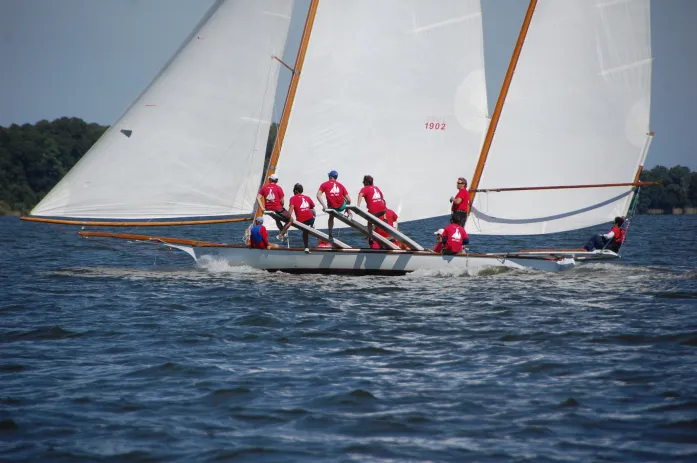
\includegraphics[keepaspectratio]{images/chapter5/watchlogcanoeraces.png}}

}

\caption{With their huge ``springboard'' planks and sprit booms, the log
canoes of the Chesapeake provide a glimpse of what the big racing
sharpies of the 1800s must have looked like. Although the log canoes
don't appear to have played a role in the development of the racing
dinghy, I'll take any excuse to include a pic of these extraordinary
veteran examples of the high-performance centreboarder.}

\end{figure}%

The speed of the long, slender New Haven sharpie soon got the attention
of yachtsmen, and soon sharpies were being built as yachts or converted
into yachts. Fittingly, it was Bob Fish who is credited with building
the first big sharpie yacht, in the shape of the 51 foot Lucky of 1855.
But sharpie yachts had limitations. The slim, shallow lines of the
sharpie meant that it pounded upwind and had limited stability, and the
high cabin tops that were needed to provide headroom increased windage
and raised the centre of gravity. At least one early sharpie builder and
fan claimed that for all their virtues (``their quickness is only
equalled by two well-matched Tom cats in a moonlight set-to''), they
were surprisingly heavy and unless over 25 ft, poor in a
seaway.\footnote{Forest \& Stream, 1879 p 14}

The man who did most to promote the sharpie to yachtsmen and minimise
its flaws was Thomas Clapham. A man of some wealth, Clapham was cruising
on his yacht (which was probably a typical New York centreboard sloop,
since she was created by sandbagger builder ``Hen'' Smedley) in 1863
when he met two brothers from Rhode Island on their home-made yacht.
Clapham challenged them to a race, which the brothers easily won.
Clapham became the first person to order a yacht from the two brothers,
thereby launching the boatbuilding career of John and Nat Herreshoff.

An easy man to like, Chapham became a lifelong friend of the Herreshoff
family. When Clapham's fortune collapsed, he moved into a smaller house
on his estate and took up boatbuilding as a career. Clapham, who had
owned a small sharpie as a boy, did more than anyone to develop the
working New Haven sharpie into a fast pleasure yacht. At a time when
science was moving into sailboat design, Clapham was a throwback to old
methods. He developed his designs by racing models on the trout pond
behind his workshop and, like the old sandbagger designers, carving
models and taking the lines off them. \footnote{Yachting, Dec 1938 p 53.}
As WP Stephens noted, he had a simple philosophy of design; he believed
that boats should sail over the water rather than carve through it, and
that a boat's fore-and-aft lines should follow segments of a circle.

Clapham's first major contributions to design were the promotion of the
yawl rig and the development of his patented ``Nonpariel Sharpie''
shape. The ``Nonpariel'' concept replaced the sharpie's shallow, flat
bottom with deep V-shaped sections. According to sharpie expert Reuel
Parker, there had been other Vee-bottom hard chine boats before (such as
the skipjack) but Clapham was the first to develop a significant degree
of deadrise and to adapt it to the faster, safer sharpie shape.

\begin{figure}[H]

{\centering \pandocbounded{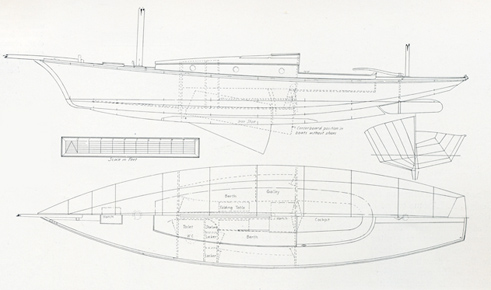
\includegraphics[keepaspectratio]{images/chapter5/sharpieplan.jpg}}

}

\caption{Thomas Clapham's ``Nonpariel Sharpie'' is sometimes claimed to
be the ancestor of most Vee-bottomed hard-chine boats.}

\end{figure}%

Clapham's sharpies demonstrated that a lightweight, lightly ballasted
boat under a moderate rig was not only fast, but more importantly, safe.
Clapham became prominent during the bitter flame wars between the fans
of the heavy, deep and narrow British cutter and the heavy, shallow and
beamy American centreboarder. He took the controversy as an opportunity
to promote his beloved sharpies (and his business building them) by
criticising both the cutter and the sloop, which he dubbed
``monstrosities, built for the sole purpose of carrying enormous rigs at
the expense of comfort, safety, and scientific principles.'' Clapham
became an effective propagandist for the light displacement boat,
claiming that the light, narrow and shallow sharpie was not only faster
but safer; ``give her a narrow beam not exceeding one-fourth her length,
and nothing is easier (when one knows how) than to produce a yacht that
shall face the roughest sea'' he boasted. \footnote{Yachting, Dec 1938 p
  53.} Clapham's outspoken promotion of the sharpie went so far that he
even became a character in a potboiler Victorian-era romantic novel, in
the guise of ``the sharpie maniac who believes that all good yachting
things are to come out of his flat-bottomed broad-beamed shallow-draught
favourites'', who was called ``the man of many sharpies'' and had
``thrown his soul into sharpies and constructed the largest and fleetest
and safest and roomiest that roam the seas.''\footnote{``Love and Luck,
  the story of a summer's loitering on the Great South Bay'' by Robert
  Barnwell Roosevelt, 1886.} Although most of Clapham's effective
publicity efforts went into his bigger boats, he made some sharpies as
small as 15 feet long but there is no evidence that any of them
raced.\footnote{``The earliest trace that I can find of small racing
  sharpie dinghies'':- a letter in the American Canoeist of December
  1882 mentioned a 16 foot Clapham sharpie on Lake Michigan that
  apparently no one, including canoe sailors, could keep upright. No
  further details or racing history have been found so far. Clapham
  later claimed that issue lay with the owner's decision to buy the
  rowboat version of his boat and fit it with a sail, but he gave no
  information about the alternative. A 15 foot long, 54in beam sharpie
  built by Clapham was also advertised as an able cruiser in Forest and
  Stream on May 17 1888. On June 21 1888 the same paper reported that
  Clapham had an order for a 20 foot racing sharpie.}

The Nonpariel was soon followed by another variation on basic sharpie,
when young boatbuilder Larry Huntington introduced a sharpie with bottom
sections that followed an arc, rather than a Vee like the Nonpariel or a
straight line like the New Haven types. It's unclear when small dinghies
started adopting the sharpie shape, and how much influence smaller
hard-chine boats like ``flatiron skiffs'' or punts had on the craft that
became known as sharpies. It's said that in 1863, a M Broca of France
visited New Haven while studying the oyster fisheries of the USA. He
sent a sharpie (possibly a small 22 footer, although most were much
longer) back home, and in the 1880s there was a belated spark of
interest in the type in France. The canoes of the USA and UK had both
experimented with ``sharpie'' hulls before 1892, but whether were
actually influenced by the New Haven type or had merely adopted the term
``sharpie'' to describe a hull shape that had been inspired by other
slender flat-bottomed craft like the old duck punts is impossible to
know.

\pandocbounded{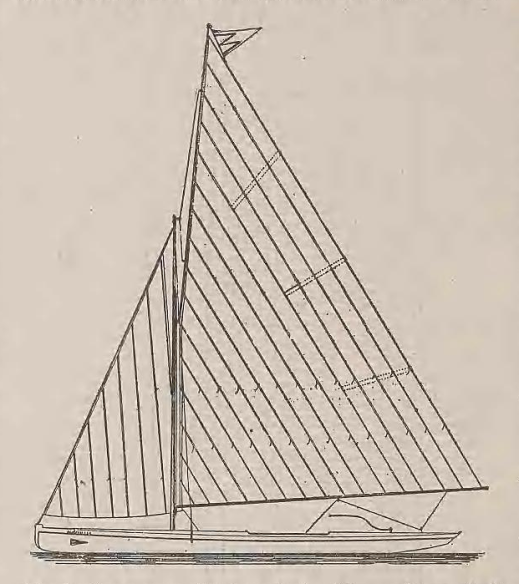
\includegraphics[keepaspectratio]{images/chapter5/french-sharpie-sailplan.png}}
\pandocbounded{
\includegraphics[keepaspectratio]{images/chapter5/french-sharpie-hull.webp}}

The earliest trace that I can find of small racing sharpie dinghies in
the English-speaking world is in the early 1890s, when Shelter Island,
across the other side of Long Island Sound from New Haven, developed a
class of 16 footers. As if to underline the difficulty of tracing the
family tree of the sharpie, the most detailed account of the Shelter
Island boats notes that ``in Gravesend bay, this type is called a
flattie, which at Shelter Island, where they are also very popular, it
is known as a sharpie.''\footnote{The Brooklyn daily Eagle, 17 May 1896
  p 15}

\begin{figure}[H]

{\centering \pandocbounded{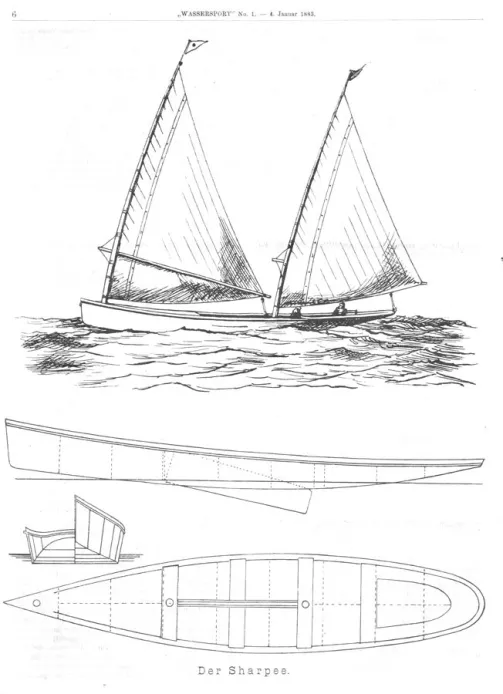
\includegraphics[keepaspectratio]{images/chapter5/wassersport-on-sharpie-21.png}}

}

\caption{A ``Sharpee'' as pictured in Germany's Wassersport magazine in
1883. This looks like an original New Haven Sharpie. The accompanying
article describing the origin of the Sharpie followed the normal tale of
its New Haven origins. From the German Yachtsportarchiv, created by
Freundeskreis Klassische Yachten e.V.}

\end{figure}%

The Shelter Island sharpies were ``nothing more than a flat bottomed row
boat, fitted with a center boat to prevent leeway, and cat rigged.The
peculiar advantage of this type is that it draws but two or three inches
of water and with the center-board up can be run right on short and the
mast unstopped. There she can be left for the night. To get under way
all that is necessary is to step the mast, the work of a minute, and
shove her off''\footnote{Ibid} By the middle of the decade, the Shelter
Island Sharpie Club's 16 footers carried big rigs (300ft2 main, 150 sq
ft spinnaker), capsized often, and the fleet included several women
skippers.

\begin{figure}[H]

{\centering \pandocbounded{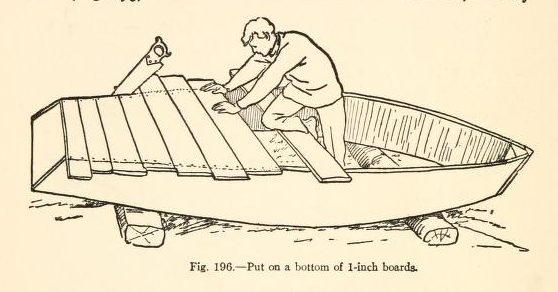
\includegraphics[keepaspectratio]{images/chapter5/sharpie-building.png}}

}

\caption{Many early sailing books promoted the sharpie as an excellent
choice for the home builder. This 12ft6in boat sailing dinghy with
1in/25mm thick planks seems to be a typical example of these simple but
heavy craft. From Boat-Building and Boating by DC Beard, 1911.}

\end{figure}%

By 1895, small sharpies were also racing across the other side of the
world in Brisbane, Australia. At least one of the early boats was
described as being ``American style'', but no further information was
included. The Brisbane sharpie movement started with as a small group of
boys racing 12 footers, but over the next decade the city developed a
thriving scene with several classes of sharpies, including 10 footers
for juniors, unrestricted 14 footers, 14 footers with restricted sail
area, and 18 footers that could run with the ``skiffs''.

Although small hard-chine training dinghies spread throughout the state,
in typical sharpie style, the Brisbane boats largely kept under the
radar and have been long forgotten. Perhaps the whole breed of early
sharpie-type racers fell between two stools; neither quite as fast as
the round bilge boats, nor cheap and simple enough to be truly popular.

\pandocbounded{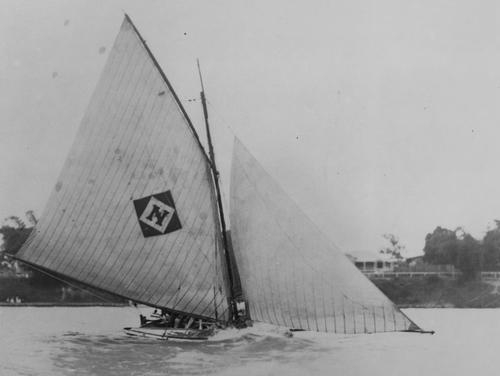
\includegraphics[keepaspectratio]{images/chapter5/nell-in-sail-on-the-brisbane-river-19161.jpg}}

\begin{figure}[H]

{\centering \pandocbounded{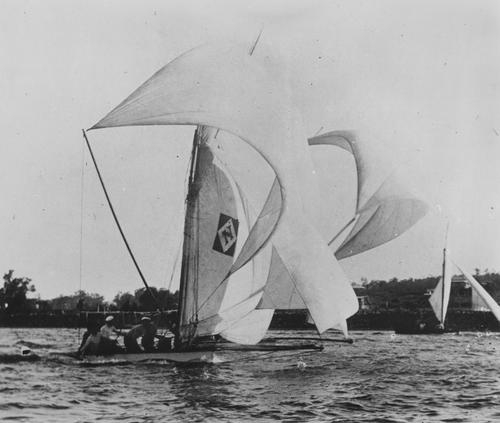
\includegraphics[keepaspectratio]{images/chapter5/nell-in-full-sail-1914.jpg}}

}

\caption{Nell, the champion 14 Foot Sharpie of Brisbane, Australia, in
1915. By then the term ``sharpie'' seems to have almost become a generic
term for a hard chine boat, especially one with narrow beam. Oxley
Library pics}

\end{figure}%

There seems to be no evidence that the Shelter Island sharpies or
similar boats had any direct influence on later hard-chine dinghies. But
there is one enormously influential class where there is strong evidence
of a link with the original New Haven sharpie -- the International Star
keelboat. George W Elder, the original class secretary and a man who
knew the Star's designer William Gardner, specifically states in his
class history ``Forty Years Among The Stars'' that the former Olympic
keelboat was derived from the New Haven sharpie, through Gardner's 1896
yacht Departure and the Bug class. The Star's arc-bottom hard shape was
then followed by such classes as the Comet (designed by a former Star
World Champion and originally labelled the Star Junior) and Lightning.

\begin{figure}[H]

{\centering \pandocbounded{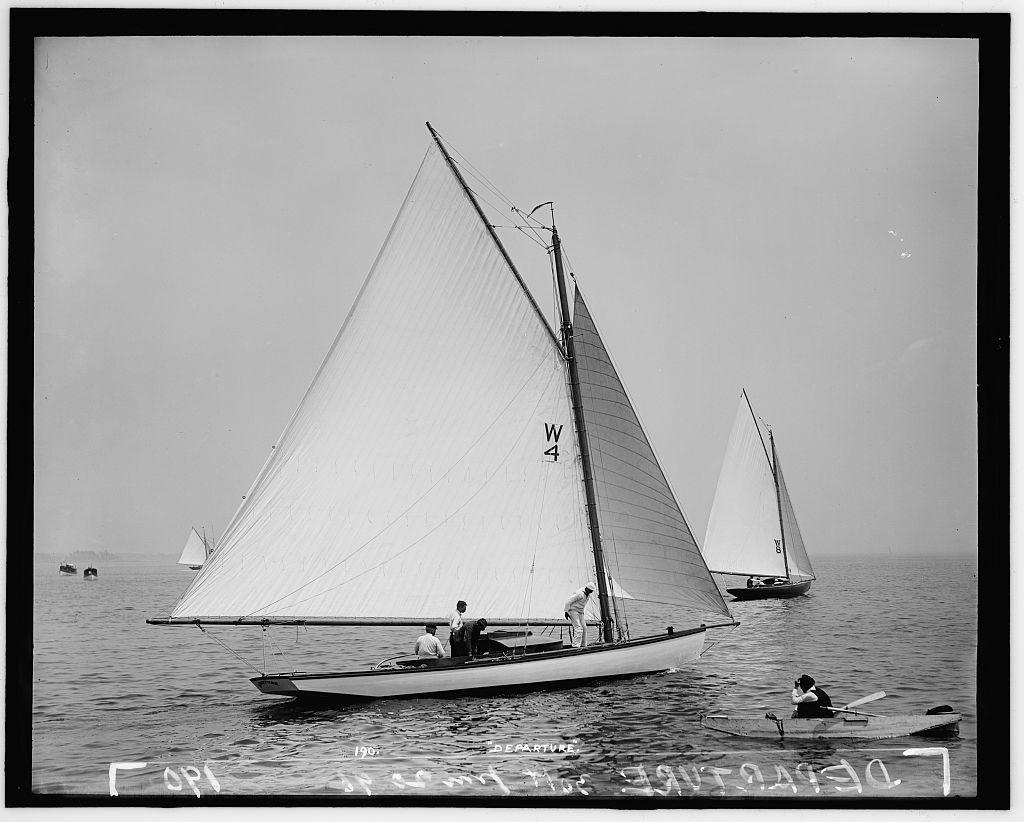
\includegraphics[keepaspectratio]{images/chapter5/departure.jpg}}

}

\caption{Departure was an ancestor of the Star, the boat that seems to
have played a significant role in spreading the sharpie and hard chine
ideas. Departure was no dinghy, but she may be significant since she was
a rare example of an early sharpie-style hard chine boat that raced in a
restricted class against conventional round-bilge boats. She was
competitive but not outstanding; perhaps an illustration that in the
days before lightweight construction, chine boats were generally
slightly slower than equivalent round-bilge designs.}

\end{figure}%

The other missing piece in the link between the New Haven Sharpie and
the later American chine dinghies was a class I'd never heard of until
sailing historian Rod Minchner posted a piece about it on his blog,
http://earwigoagin.blogspot.com.au/. The 15 foot long Cricket evolved
around Atlantic City in the 1890s, boomed in that area around 1900, and
then moved south to the Miami area where it survived until the 1950s. It
then vanished with so little trace that even Minchner's research has
failed to uncover its designer and details about its early history.

\begin{figure}[H]

{\centering \pandocbounded{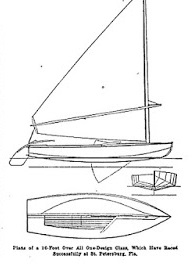
\includegraphics[keepaspectratio]{images/chapter5/florida_one_design.jpg}}

}

\caption{The One Design class for St Petersburg YC is believed to have
been similar to the Cricket. Plans from The Rudder magazine, thanks to
Rod Minchner's earwigoagin.blogspot.com.au}

\end{figure}%

So why does this long-gone local class seem to be so important? It's
because the Cricket seems to show another clear link between the early
sharpies and the later hard-chine Vee-bottom dinghies that formed the
backbone of US dinghy sailing for decades. The Cricket definitely has
strong sharpie DNA -- it carried a freestanding rig with a sprit boom
and ``pry board'' like the early New Haven racing sharpies. But the
Cricket's deep Vee single-chine hull is also very similar to that of
later boats like the Snipe and California's Snowbird, which played such
major roles in dinghy sailing from the 1920s to the current day.

And so in the end, it seems clear (as we'll get to in more detail later)
that hard chine dinghies in other areas evolved completely independently
from the sharpie. But it also seems clear that while the sharpie story
never had a star like Una or Truant, the original New Haven sharpie did
have a strong influence on the design of the hard chine dinghies of the
USA. And it seems clear that one of those classes, the Cricket, went on
to inspire one of the most influential boats in the history of dinghy
design. But that's for a later post\ldots{}

\bookmarksetup{startatroot}

\chapter*{References}\label{references}
\addcontentsline{toc}{chapter}{References}

\markboth{References}{References}

\phantomsection\label{refs}




\end{document}
